\chapter{Avalia\c{c}\~{a}o Experimental} \label{chap:avaliacao}
Neste capítulo são descritos os experimentos realizados para a validação deste trabalho.

A realização do monitoramento dos sinais motores de uma maneira não-invasiva é um desafio, logo esta tese fornece uma forma lúdica de monitorar os dados de saúde por meio de jogos eletrônicos que podem ser integrados à rotina diária dos usuários. %Pois, a partir de um \textit{HGMS-E} é possível capturar, processar e classificar os movimentos cinéticos exercidos pelos usuários.

%Sabendo que o acompanhamento de sinais motores, integrados à rotina diária do paciente traz benefícios ao tratamento e qualidade de vida do mesmo do ponto de vista do profissional da saúde. Por intermédio desse trabalho, conseguimos capturar dados motores utilizando sensores de movimento. Esses dados permitem auxiliar no acompanhamento de doenças com comprometimento motor tal como o~\ac{dp}. Então, neste trabalho nós desenvolvemos um mecanismo de de captura de dados motores embutidos num jogo eletrônico, o qual permite monitorar e quantificar os sinais motores de uma forma lúdica e não-invasiva.




\section{ETAPA 1 - Entrevista Semiestruturada com Profissionais de Saúde}\label{chapter:entrevista_semi_estruturada}

A interpretação de dados é o cerne da pesquisa qualitativa, esse método tem como função desenvolver a teoria, servindo ao mesmo tempo de base para a decisão sobre quais dados adicionais devem ser coletados, por meio de codificação seletiva~\cite{FLI04}. Esta técnica, permite elaborar uma categorização nos dados, demonstrando ao pesquisador quais são os fenômenos mais preponderantes da pesquisa. O procedimento da interpretação dos dados, assim como a integração de material adicional são encerrados quando se atinge a "saturação teórica", ou seja quando o avanço na codificação não resulta na aquisição de novos conhecimentos~\cite{FLI04}.

Para análise dos textos provenientes da pesquisa foram transcritos as entrevistas com: neurologistas e fisioterapeutas especialistas em neurologia. Com  a codificação seletiva foi possível categorizar os as ocorrências de acordo com o conteúdo de cada texto. Ou seja, as respostas de cada participante foram analisadas incluídas na árvore de categorias como sugere o método de pesquisa~\cite{FLI04}. 

Para auxiliar no processo de: análise, seleção e codificação. Foi utilizado uma ferramenta de suporte à pesquisa qualitativa (\textit{QDA Miner}~\cite{qda13}), por meio desta, foi possível categorizar e reformular a árvore de categorias~\cite{FLI04} diversas vezes durante o processo de análise~\cite{FLI04}.


\subsection{Objetivo da Pesquisa}
O objetivo da entrevista semiestruturada~\cite{FLI04} foi entender como é feito o acompanhamento do paciente com sintomatologia do~\ac{dp}, juntamente aos profissionais de saúde: neurologistas que prescrevem a dosagem medicamentosa e fisioterapeutas que fazem o tratamento  de reabilitação e acompanhamento motor do paciente. Esse profissionais de saúde, foram indagados se haveria melhora na tomada de decisão caso estes pudessem acompanhar os sinais motores em diariamente. Procurou-se encontrar dentro do contexto de estudo, a importância do monitoramento de dados de saúde e os benefícios trazidos por este.

As entrevistas foram realizadas presencialmente, com perguntas não estruturadas e, com uma maior estruturação no decorrer da entrevista preocupando-se em evitar a referência do entrevistador sobre os pontos de vista do entrevistado, conforme sugere o método científico~\cite{FLI04}. 

\subsubsection{Instrumento de Análise dos Dados da Pesquisa Qualitativa} \label{section:analise_dados} 
A pesquisa qualitativa assistida por computador permite uma melhor categorização das informações obtidas em modo texto. O \textit{software} QDA Miner~\cite{qda13} auxilia o pesquisador na organização dos registros da pesquisa e das interpretações dos mesmos, justificando-se o uso da ferramenta devido a dificuldade de classificar e analisar os dados obtidos. Nessa análise, foram consideradas as atividades referentes ao acompanhamento dos sinais motores em pacientes com~\ac{dp}. Buscou-se durante a pesquisa avaliar se um cenário de monitoramento dos sinais motores por meio de jogos eletrônicos auxiliaria os profissionais de saúde quanto ao tratamento de seus pacientes.

Nesta seção, faz-se um detalhamento do resultado da entrevista semiestruturada, descrevendo a opinião dos entrevistados e coletando requisitos baseado nas necessidades expostas pelos mesmos. Por meio desta etapa da pesquisa foi avaliada a \textbf{ETAPA 1} da pesquisa: \textit{Quais os benefícios de acompanhar diariamente os sinais motores do paciente do ponto de vista do profissional da saúde}.

%	\begin{description}

%	\item[H1] O acompanhamento de sinais motores integrados à rotina diária do paciente, traz benefícios ao tratamento e na qualidade de vida do mesmo, do ponto de vista do profissional da saúde.
% 	\end{description}
	
%\subsubsection{Análise da Entrevista Semi-Estruturada}
%A análise qualitativa ~\cite{FLI04} permite identificar as práticas dos profissionais de saúde referentes ao acompanhamento dos sinais motores em pacientes de parkinson e como essas práticas podem ser aperfeiçoadas num cenário em que haja o monitoramento dos sinais. 


\subsection{Perfil dos Participantes}
O perfil dos participantes é composto por quatro profissionais da saúde, dos quais: dois são fisioterapeutas com especialização em neurologia, e dois são médicos neurologistas. A escolha desse perfil se fez de acordo com seus ofícios e responsabilidades e complementaridade quanto ao tratamento do paciente. Os neurologistas realizam o diagnóstico e acompanham os sinais motores juntamente com as informações obtidas do paciente ou de seu cuidador, e baseado nas informações realiza o gerenciamento da dosagem medicamentosa da doença. Por outro lado, os fisioterapeutas fazem o acompanhamento dos sinais motores em sessões de fisioterapia promovendo a aprendizagem motora desses pacientes. Logo, esses profissionais possuem visões e preocupações distintas e inerentes a seu ofício. 

Para manter a confidencialidade de informação, os entrevistados receberam uma \textbf{LEGENDA} que identifica o perfil profissional seguido por um número sequencial, o qual identifica o entrevistado mas preserva sua identidade (Tabela~\ref{table:perfil_analise_participantes}).

\begin{table}[h]
\caption{Perfil dos Participantes}
\label{table:perfil_analise_participantes}
\begin{tabular}{|l|l|c|c|}
\hline
\textbf{LEGENDA} & \textbf{PROFISSÃO}             & \multicolumn{1}{|l}{\textbf{IDADE (ANOS)}} & \multicolumn{1}{|l|}{\textbf{EXPERIÊNCIA (ANOS)}} \\ \hline
FIS\_01          & Fisioterapia em Neurologia & 40                                         & 10                                                \\ \hline
FIS\_02          & Fisioterapia em Neurologia     & 39                                         & 10                                                \\ \hline
NEU\_01          & Médico Neurologista            & 42                                         & 15                                                \\ \hline
NEU\_02          & Médico Neurologista            & 67                                         & 30                                                \\ \hline
\end{tabular}

\end{table}

\subsubsection{Questionário de Pesquisa}
Para a formulação do questionário foram realizadas análises nas diretrizes médicas ~\cite{protpar010,national2006parkinson} e na tabela UPDRS ~\cite{updrs87} sobre o progresso da ~\ac{dp} e dos sinais monitoráveis por sensores de movimento. Para a entrevista foram elaboradas 15 perguntas agrupadas em 3 seções (Apêndice \ref{apendice:entrevista-semi-estruturada}) com os seguintes temas: sinais do~\ac{dp}, monitoramento da saúde motora e os benefícios advindos do monitoramento. Onde o entrevistador selecionou as questões de acordo com o perfil profissional.

\subsection{Análise}
Durante a análise das entrevistas foram extraídos fragmentos, e a nomenclatura utilizada contém o prefixo \textbf{FRAGMENTO} mais um número sequencial identificando o mesmo. Esse procedimento permite identificar \textbf{requisitos} que orientem a proposta de monitoramento de dados motores por intermédio de jogos eletrônicos. Logo, os requisitos extraídos nesta abordagem foram obtidos a partir da perspectiva do profissional de saúde em relação ao tratamento e acompanhamento da~\ac{dp}. 

\subsubsection{Diagnóstico}\label{section:analise_diagnostico}

Na entrevista junto aos neurologistas, foi indagado como o diagnostico da~\ac{dp} é realizado.  A entrevista corroborou com a literatura médica~\cite{tolosa06,vedolin2003} em relação ao diagnóstico de exclusão do \ac{dp}~\cite{protpar010,national2006parkinson}.  

Todos os profissionais informaram que o sintoma mais comum é o tremor de repouso, e que este inicialmente é unilateral e seguido de uma bradicinesia como podemos perceber nos ([FRAGMENTO-01][FRAGMENTO-02]). Ainda no ([FRAGMENTO-01]), existe uma ocorrência do \textbf{[NEU\_01]} em que o mesmo evoca sobre a importância da técnica de \textit{Finger Taps} ~\cite{updrs87} para avaliação da bradicinesia.


\begin{quote}
\textbf{[FRAGMENTO-01][NEU\_01]} - 
\emph{
O diagnóstico da doença de Parkinson é quando o paciente chega se queixando de tremor. Esse sintoma começa com um tremor unilateral geralmente pelas mãos, lentamente progressivo e de repouso. Além do tremor esse paciente exibe também uma lentidão que a gente consegue detectar pelo \textit{Finger Taps}. Essa técnica consiste em tocar o polegar ao primeiro e segundo dedo simultaneamente para ver se há ou não lentidão. Faz-se uma comparação sempre com o outro lado para visualizar possíveis diferenças. 
Existe também uma rigidez no braço, quando faz-se uma flexão e extensão do membro e percebe-se que o tônus desse paciente comparado com o outro lado exibe uma diferença.
}
\end{quote}

\begin{quote}
\textbf{[FRAGMENTO-02][NEU\_02]} -
\emph{
O diagnóstico da doença de Parkinson é feito com uma das queixa iniciais do paciente é um tremor de repouso, geralmente associado a uma dificuldade na marcha. Então normalmente os pacientes reclamam de uma perna presa e um tremor de repouso. 
}
\end{quote}

Uma ocorrência no ([FRAGMENTO-03]) que deve ser ressaltado, é o que o entrevistado referiu como ``\textit{boa resposta ao prolopa}''. Essa ocorrência é denominada de diagnóstico diferencial da \ac{dp} ~\cite{protpar010}, consiste na redução dos sinais parkinsonianos em decorrência da resposta ao tratamento medicamentoso. 

\begin{quote}
\textbf{[FRAGMENTO-03][NEU\_01]} - 
\emph{
Então os sinais é o tremor em repouso, a lentidão e a rigidez. Inicialmente apenas de um lado, por exemplo começa no braço direito e depois vai para a perna direita, depois para o braço esquerdo e depois a perna esquerda. Isso lentamente progressivo, a gente faz a exclusão com outras doenças através de outros exames como tomografia, ressonância ou a uma boa resposta ao prolopa.
}
\end{quote}

\subsubsection{Sintomas}
Nesta seção estão expostos sinais para o acompanhamento da sintomatologia da ~\ac{dp}.

%\subsubsection{Tremor}
O sintoma de tremor, além de ter sido referenciado durante o diagnóstico da doença na Seção ~\ref{section:analise_diagnostico} por todos os entrevistados, possui particularidades como a dificuldade de controlar o sintoma por intermédio do tratamento medicamentoso ([FRAGMENTO-04]), e não é tão incapacitante quanto a bradicinesia ~\ac{dp}. No ([FRAGMENTO-05]) o [NEU\_01] reforçou sobre a importância de controlar os sinais de lentidão do movimento ante os de tremor ~\cite{do2007parkinson}.

\begin{quote}
\textbf{[FRAGMENTO-04][NEU\_01]} - 
\emph{
Mas a gente tem que ver, porque as vezes o tremor é muito mais difícil de você controlar. Porque está relacionada ao emocional do paciente. Quanto mais emocionalmente desequilibrado o paciente tiver, mais tremor ele tem.
}
\end{quote}

\begin{quote}
\textbf{[FRAGMENTO-05][NEU\_01]} - 
\emph{
O controle do tremor é um pouco complicado porque é um sintoma mais difícil de ser controlado com as medicações que temos hoje.  Então você poderia ver nesse seu projeto a lentidão. Porque o paciente quer tremer mas ele não quer ficar lento.
}
\end{quote}


%\subsubsection{Bradicinesia}\label{section:analise_bradicinesia}

O pesquisador indagou se o sintoma da bradicinesia era considerado o mais debilitante da ~\ac{dp} e como resposta ele obteve a afirmação de que a bradicinesia impacta diretamente na qualidade de vida do paciente, privando-o de realizar atividades diárias ([FRAGMENTO-06]).

\begin{quote}
\textbf{[FRAGMENTO-06][NEU\_01]} - 
\emph{
É ele atrapalha né, principalmente no levantar no andar, para você se levantar, pentear o cabelo o tremor é prejudicial. Porém mais prejudicial ainda é a lentidão do movimento.
}
\end{quote}

Ao indagar se o movimento de adução e abdução do braço seria relevante para a identificação da~\ac{dp}, o [NEU\_01] informou que a bradicinesia é um sintoma que traz lentidão em todo o corpo e possivelmente seria afetada por este movimento. Pois, devido à redução dos movimentos automáticos ([FRAGMENTO-07]), traz outros impactos físicos ao paciente ([FRAGMENTO-08]).

\begin{quote}
\textbf{[FRAGMENTO-07][NEU\_01]} - 
\emph{
Na verdade o movimento em si, vai ver o quão lento está. Porque você não tem um déficit motor. O comprometimento na doença de Parkinson está no comprometimento piramidal, o comprometimento extra-piramidal não vai estar alterando a força motora. O que vai estar vai ser exatamente a lentidão. Por exemplo, é um paciente que está andando você que os movimentos dele automáticos estão reduzidos, principalmente no balançar dos braços. Você vai andando, vai andando, você vê aquele paciente que está com a força, ele está com toda a estrutura piramidal tudo normal. Mas ela anda lento em consequência da lentidão do movimento porque os movimentos automáticos estão reduzidos.
}
\end{quote}


\begin{quote}
\textbf{[FRAGMENTO-08][FIS\_01]} - 
\emph{
Os sinais mais frequentes a gente tem a bradicinesia que é a lentificação do movimento, a gente tem um padrão postural que começa a ficar bem nítido que o paciente apresentar o Parkinson. Você percebe uma perda da movimentação automática da cintura escapular e aí ele começa a apresentar uma diminuição no volume da voz que é uma diplofonia, e apresenta uma maior rigidez muscular. Eles reclamam bastante e a bradicinesia que tornam os movimentos cada vez mais lentos.
}
\end{quote}

%\subsubsection{Marcha}
% Foi identificada uma ocorrência na dificuldade do andar do paciente de~\ac{dp}, quando o [NEU\_01] cita no ([FRAGMENTO-07]) (``\textit{Você vai andando, vai andando, você vê aquele paciente que está com a força, ele está com toda a estrutura piramidal tudo normal. Mas ela anda lento em consequência da lentidão do movimento ...}''. O [NEU\_02] corrobora com a mesma opinião ao citar a dificuldade de iniciar a marcha no ([FRAGMENTO-09]). O fisioterapeuta no papel de realizar o acompanhamento da marcha nas sessões fisioterápicas, fornece um aprendizado motor para a melhora da qualidade de vida do paciente de acordo com suas limitações ([FRAGMENTO-10]).
% 
% \begin{quote}
% \textbf{[FRAGMENTO-09][NEU\_02]} - 
% \emph{
% Problema na marcha. Dificuldade de iniciar a marcha, certa dificuldade de um lado comprometido. Mesmo quando o sintoma está unilateral eles sentem dificuldade para iniciar a marcha.
% }
% \end{quote}
% 
% \begin{quote}
% \textbf{[FRAGMENTO-10][FIS\_01]} - 
% \emph{
% Numa marcha, o doente de Parkinson tem a tendência de estar olhando para o chão. Mas a gente sabe que isso não é compatível com uma boa marcha a tendência é cair, para piorar eles têm os passos miúdos e também um passo arrastado. Então esse passo favorece a queda, poise ele perdeu a marcha automática que é aquela que a gente adquire na infância. O que a gente faz nas sessões de fisioterapia é tentar aplicar auto-correções para adaptar o paciente à nova realidade para que ele tenha uma aprendizado motor e no futuro um automatismo do movimento.
% }
% \end{quote}
% 
% Devido a quantidade de ocorrências sobre a análise da marcha para o acompanhamento da ~\ac{dp}, e a possibilidade da ocorrência de quedas dos indivíduos. Esses, dois fatos corroboraram com o uso de base de dados contendo dados sobre a marcha, pois isto vai além do custo financeiro para a aquisição dos sensores que capturam a ~\ac{fvrs}. Logo, ao usar bases contendo esses dados para a pesquisa, preserva-se a integridade física dos pacientes.



\subsubsection{Monitoramento Motor}
Nesta seção está exposta a importância do monitoramento dos sinais capturados no estudo analítico de caso controle definido no método de pesquisa na Seção~\ref{section:estudo_caso_controle}. Nesse estudo também pretende-se identificar as características dos movimentos que possam ser extraídos desses sinais, e que venham fornecer subsídios para diferenciar indivíduos diagnosticados com~\ac{dp} ante indivíduos sem o diagnóstico.

%\subsubsection{Amplitude do Movimento dos Braços}

Ao indagar ao [FIS\_02] se o movimento de adução e abdução do braço seria relevante para a identificação da~\ac{dp}, este informou que mesmo não sendo um teste específico para a identificação da doença, existem diferenças significativas encontradas em indivíduos diagnosticados com parkinson [FRAGMENTO-11].
\begin{quote}
\textbf{[FRAGMENTO-11][FIS\_02]}-
\emph{
Sim. Existe alterações sim, mas eu nunca vi especificamente esse teste como sendo usado para diagnóstico da doença. Mas que realmente existem mudanças no movimento de adução e abdução de uma pessoa normal ante a um parkinsoniano.
}
\end{quote}

O [FIS\_01], explicou os motivos que levam a perda da mobilidade no movimento de adução e abdução ([FRAGMENTO-12]) e consequentemente, reforça que esse movimento poderia ser monitorado para verificar o comprometimento da doença. Em um outro fragmento ([FRAGMENTO-13]) o mesmo fisioterapeuta menciona a importância de monitorar a amplitude do movimento, pois permite visualizar a resposta do paciente ao tratamento oferecido.

\begin{quote}
\textbf{[FRAGMENTO-12][FIS\_01]}-
\emph{
Têm, porque uma das grandes perdas que eles apresentam é na cintura escapular e consequentemente é pegando a parte de ombro. Pois caso ela seja mais fixa, porque geralmente o paciente de Parkinson abduz o ombro. O ombro fica abduzido junto ao tronco e ai ele perde a mobilidade do cotovelo e punho e também o movimento fica comprometido por conta disso.
}
\end{quote}

\begin{quote}
\textbf{[FRAGMENTO-13][FIS\_01]}-
\emph{
Mesmo sabendo que a tendência é uma lentificação (bradicinesia).  As outras doenças também, porque um dos objetivos nossos é o aumento da amplitude. Então é um meio interessante para a gente conseguir visualizar se o tratamento está dando certo ou não.
}
\end{quote}



\subsubsection{Velocidade do Movimento De Adução e Abdução dos Braços}
Um ponto de convergência, entre os profissionais entrevistados, é a importância de monitorar a velocidade angular dos pacientes. Os profissionais tentam associar o tratamento fisioterápico e medicamentoso para a melhora da bradicinesia. Logo, para estes profissionais a melhora está condicionada a um aumento na velocidade do movimento ([FRAGMENTO-14],[FRAGMENTO-15])

\begin{quote}
\textbf{[FRAGMENTO-14][NEU\_01]} - 
\emph{
É como eu falei para mim seria melhor se capturássemos se ele está mais lento. Se através dessa amplitude você conseguir por intermédio do computador identificar que ele está mais lento de um lado do que do outro, e conseguir visualizar a velocidade de um lado e do outro. Então isso é interessante.
}
\end{quote}


\begin{quote}
\textbf{[FRAGMENTO-15][FIS\_01]} - 
\emph{
É e consequentemente a velocidade, porque nesse caso o tratamento é diretamente relacionado a isso quanto mais veloz o parkinsoniano é melhor para a gente melhor prognóstico a gente pode ter lá na frente. Mesmo sabendo que a tendência é uma lentificação.
}
\end{quote}

%\subsubsection{Assimetria do Movimento}

A assimetria do movimento acomete os pacientes que estão nos estágios iniciais da doença. Por esse motivo, geralmente ela é identificada durante o diagnóstico [FRAGMENTO-03]. Porém, alguns pacientes parkinsonianos apresentam a assimetria do movimento quando um dos lados é mais comprometido que o outro. Por essa razão é que o [NEU\_01] afirmou \textit{``Se através dessa amplitude você conseguir por intermédio do computador identificar que ele está mais lento de um lado do que do outro''}. Pois, a tendência natural da evolução da ~\ac{dp} é a redução na assimetria do movimento conforme a opinião do [NEU\_01] no [FRAGMENTO-16] e na tabela UPDRS ~\cite{updrs87} em sua escala de avaliação do progresso da doença (Seção ~\ref{section:escalas_avaliacao}).

\begin{quote}
\textbf{[FRAGMENTO-16][NEU\_01]}-
\emph{
No início. Geralmente o paciente se queixa de uma diminuição de força de um lado do corpo. Mas na progressão, ele vai sentir dificuldade global. Mas aqueles parkinsonianos iniciais geralmente eles se queixam na diminuição do movimento de um dos lados.
}
\end{quote}

\subsubsection{Benefícios Advindos do Monitoramento}


%\subsubsection{Quantificação dos Sintomas}
Em relação aos benefícios advindo do monitoramento pudemos identificar: a quantificação dos sinais motores, amplitude de movimento de adução e abdução do braço,  velocidade angular destes movimentos. Essa análise trouxe dois grupos de respostas: o primeiro reconhecia da importância da quantificação dos dados para identificar a melhora ou piora do paciente [FRAGMENTO-17], e outro relatava que essa informação tinha mais validade científica do que prática [FRAGMENTO-18]. Todavia, caso esses profissionais tivessem acesso a um sistema que permitisse o monitoramento motor, possivelmente eles iriam perceber os benefícios da abordagem e modificar sua prática atual ao adotar uma nova proposta.

\begin{quote}
\textbf{[FRAGMENTO-17][FIS\_02]}-
\emph{
É preciso ter parâmetros sim. Pois atualmente usamos muito o olho clínico e ai vai de cada profissional. Se tivermos números facilitam bastante porque se tornam fatos e basearmos nossas conclusões em números é bem melhor.
}
\end{quote}

\begin{quote}
\textbf{[FRAGMENTO-18][FIS\_01]}-
\emph{
É interessante em termos de pesquisa. Em termos de clínica a geralmente a gente vai no geral. Por exemplo: Eu faço uma flexão de ombro com bastão e anotei no meu exame que ele ia até mais ou menos 70º e após 15 dias eu vejo que ele está levantando acima de 90º. Então está marcado a minha evolução. Então eu faço a avaliação nesse sentido. Então esse sistema seria bom para pesquisa mesmo.
}
\end{quote}

%\subsubsection{Gerenciamento da Dosagem Medicamentosa}
Indagou-se aos profissionais se o monitoramento dos sinais motores auxiliaria no gerenciamento da dosagem medicamentosa. Os profissionais informaram que sentem a necessidade de visualizar a eficácia do tratamento diante do paciente. O [FIS\_01] no [FRAGMENTO-19] cita a importância de avaliar tanto o tratamento medicamentoso quanto se a sua atividade fisioterápica traz benefícios ao paciente. Os neurologistas citam ([NEU\_01] e [NEU\_01]) a importância de reajustar a dosagem medicamentosa e que a quantificação do sintoma identifica o resultado do efeito medicamentoso. Outra opinião bastante pertinente é que o agravamento da ~\ac{dp} é bastante sutil do ponto de vista do [NEU\_01] no [FRAGMENTO-21]. Logo se for possível, mostrar a evolução da doença em períodos mais longos, o tratamento seria mais efetivo e, consequentemente, traria uma melhor qualidade de vida aos pacientes.

\begin{quote}
\textbf{[FRAGMENTO-19][FIS\_01]} - 
\emph{
 É interessante porque teremos uma ideia de até que ponto a medicação está sendo efetiva, até quando a patologia está progredindo e também avaliar se o nosso tratamento fisioterápico está dando resultados ao tentar frear a evolução da doença.
}
\end{quote}


\begin{quote}
\textbf{[FRAGMENTO-20][NEU\_02]} - 
\emph{
Sim. Dentro do que você propõe. Com certeza sim. Essa avaliação desses movimentos. Porque a gente consegue visualizar se a medicação está surtindo efeito, se precisa ser reajustada.
}
\end{quote}

\begin{quote}
\textbf{[FRAGMENTO-21][NEU\_01]} - 
\emph{
Se esse mecanismo acontecesse. Você poderia avaliar a dosagem de um paciente por exemplo. Veja avalie durante uma semana, não melhorou. Então a gente poderia fazer um teste com tremor, lentidão e a rigidez, se houvesse esse aspecto.  A gente poderia aumentar a dosagem e visualizaria a eficácia da dosagem com o decorrer do tempo, com o decorrer da evolução. E verificaria se realmente o paciente está melhorando. Porque o paciente da doença de Parkinson ele piora lentamente, as vezes é tão sutil que o próprio paciente não consegue. Então é como eu disse, cada paciente a evolução é diferente num existe. Mas poderia assim, se você conseguisse detectar as amplitudes do tremor por exemplo.
}
\end{quote}


\subsection{Requisitos Identificados}
A \ac{er} é o processo de descobrir o propósito do software, identificando os principais envolvidos do sistema com suas respectivas necessidades e documentando a análise para uma implementação posterior \cite{bas00}. Contudo, é um processo que deve ser continuamente repetido para que as necessidades dos envolvidos sejam satisfeitas. As técnicas para identificação de requisitos são derivadas principalmente das ciências sociais, que se baseiam em pesquisa qualitativa onde são analisados a teoria do objeto de estudo com a experiência prática dos envolvidos na pesquisa ~\cite{elicquest05,zowghi2005}.

A identificação dos requisitos de um sistema representa o início da elicitação das necessidades da solução proposta. Então, os requisitos definem quais serão os serviços que o sistema deve prover além de um conjunto de restrições existentes na operação do mesmo \cite{sommerville2011}. A técnica utilizada para a identificação dos requisitos desta pesquisa é baseada em pesquisa qualitativa, onde usou-se a entrevista semiestruturada na qual o entrevistador possui um conjunto de perguntas pré-definidas e guia a entrevista de acordo com a opinião do entrevistado~\cite{FLI04}. Ficou definido, que cada requisito deve ser importante para os entrevistados e a nomenclatura estabelecida é de \textbf{REQ-ENTREVISTAS} seguida por um número sequencial correspondente à sua apresentação. Para demonstrar a relevância dos requisitos, a teoria foi confrontada com o que é aplicado na prática pelos profissionais de saúde, por esse motivo, foram citadas referências científicas que corroboram com a análise. 



%O uso do termo "Engenharia" implica que técnicas sistemáticas e repetidas devem ser aplicadas para certificar que os requisitos de um sistema estejam completos, consistentes e relevantes \cite{sommerville2011}. O emprego correto da Engenharia de Requisitos é um passo fundamental para o desenvolvimento de um bom  produto, onde a satisfação do usuário deve ser o principal objetivo a ser atingido \cite{zowghi2005}.

\begin{description}
	\item[REQ-ENTREVISTAS-01 :] Identificar e quantificar o tremor parkinsoniano ~\cite{tolosa06,keijsers2006,lemoyne2010}.
	\item[REQ-ENTREVISTAS-02 :] Identificar a bradicinesia ~\cite{patel_monitoring_2009}. %Para identificar a bradicinesia pode ser calculada a velocidade angular do movimento de abdução e adução do braço.
	\item[REQ-ENTREVISTAS-03 :] Avaliar bradicinesia usando~\textit{finger-tapping}~\cite{finger2012}.
	\item[REQ-ENTREVISTAS-04 :] Considerar e identificar a assimetria do movimento nos estágios iniciais ~\cite{national2006parkinson}.	%Além da velocidade angular podemos calcular a amplitude do movimento, assim identificarems a assimetria do movimento com mais clareza.
	\item[REQ-ENTREVISTAS-05 :] Fornecer mecanismos para possibilitar o Diagnóstico Diferencial \cite{protpar010} da Doença de Parkinson. %caso os sinais de bradicinesia e marcha sejam identificados. Caso os indivíduos venham a surtir efeito ao medicamento e consequentemente reduzir a gravidade do sintoma, então foi possível realizar um diagnóstico diferencial.
	\item[REQ-ENTREVISTAS-06 :] Analisar a Marcha ~\cite{gaitusingsensorsreview2012}. Medir a marcha e comparar o padrão do movimento com indivíduos com e sem o diagnóstico da ~\ac{dp} para classificar a marcha como saudável ou parkinsoniana.
	\item[REQ-ENTREVISTAS-07 :] Calcular e armazenar a amplitude do movimento de adução e abdução dos braços, para realizar o monitoramento da saúde motora e poder acompanhar o tratamento.
	\item[REQ-ENTREVISTAS-08 :] Calcular e armazenar a velocidade angular do movimento de adução e abdução dos braços. Para poder avaliar o sintoma da bradicinesia.
	\item[REQ-ENTREVISTAS-09 :] Avaliar estado emocional baseado na ocorrência e comprometimento do tremor. 
\end{description}



\subsubsection{Inviabilidade Técnica}
Alguns requisitos identificados não podem ser implementados com a tecnologia de sensor de movimento usada nesse trabalho. A importância destes requisitos é reconhecida e pode ser implementada em trabalhos futuros, desde que as barreiras tecnológicas sejam resolvidas como descrito:
\begin{figure}[!h]
 \centering
 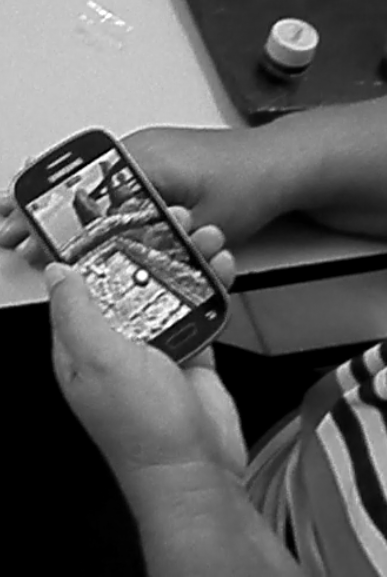
\includegraphics[scale=0.5]{./img/gametremor.png}
 % matrixargseg.png: 296x162 pixel, 100dpi, 7.52x4.11 cm, bb=0 0 213 117
 %\caption{Estágio desenvolvimento de jogos ~\cite{fullerton2008game}}
\caption{Teste de um jogo usando acelerômetro para quantificação do sinal de tremor do Parkinson}
%  \caption{Estágio desenvolvimento de jogos}
 \label{fig:gametremor}
\end{figure}

\begin{itemize}
  \item O \textbf{REQ-ENTREVISTAS-01}, o tremor de repouso é um dos principais sinais do~\ac{dp}. Sabíamos da sua importância, inclusive foi desenvolvido um jogo para \textit{Smartphone} que pudesse quantificar o tremor (Figura ~\ref{fig:gametremor}). Porém, no teste junto aos usuários, foi percebido que no momento do uso os pacientes parkinsonianos cessavam o tremor, inviabilizando assim sua quantificação. 
	\item O \textbf{[REQ-ENTREVISTAS-03]}, a técnica de \textit{finger-tapping} não pode ser avaliadas utilizando o MS-Kinnect 1.0, pois nessa versão não existe a captura do movimento dos dedos, conforme ilustrado na Figura~\ref{fig:articulacoeskinnect}.
	\item O \textbf{REQ-ENTREVISTAS-09}, por envolver estado emocional e parâmetros que não estamos levando em consideração nesse trabalho, esse requisito está fora do escopo. Entretanto, com mecanismos de detecção de batimentos cardíacos presente em versões mais atuais do MS-Kinnect, pode ser averiguada a relação dos batimentos cardíacos com o tremor.
\end{itemize}


%Em estudos prévios da nossa pesquisa, pudemos identificar esse fenômeno junto aos pacientes do~\ac{dp}, onde percebemos que os pacientes de~\ac{dp} cessavam o tremor quando confrontados com um jogo para celular desenvolvido com o propósito de quantificar o sinal do tremor (Figura~\ref{fig:gametremor}). Por esse motivo, resolvemos trabalhar com outro sinal do~\ac{dp} como a bradicinesia~\cite{protpar010} o qual pode ser avaliado utilizando um sensor de movimentos como o \textit{Ms-Kinnect Versão 1.0}~\cite{kinnect2013}. %que não necessita do contato físico do usuário além de ser utilizado em jogos eletrônicos. 



\subsubsection{Matriz de Rastreabilidade - Fragmento x Requisitos}
%\begin{center}
%\begin{table}[!htbp]
\begin{table}[!htb]
\caption{Matriz Rastreabilidade: Fragmento x Requisitos}
\label{table:matrix_rastreabilidade}
\begin{tabular}{||p{6.06cm}||ccccccccc|}
\hline
 \multicolumn{1}{|p{6.06cm}|}{\centering \textbf{FRAGMENTOS / REQUISITOS}} &  01 &  02 &  03 &  04 &  05 &  06 &  07 &  08 & 09 \\ 
\hline 
 \multicolumn{1}{|p{6.06cm}|}{\centering 01} &  x &  x &  x &  x &   &   &   &   &  \\ 
 \multicolumn{1}{|p{6.06cm}|}{\centering 02} &  x &   &   &   &   &  x &   &   &  \\ 
 \multicolumn{1}{|p{6.06cm}|}{\centering 03} &  x &  x &   &  x &  x &   &   &   &  \\ 
 \multicolumn{1}{|p{6.06cm}|}{\centering 04} &  x &   &   &   &   &   &   &   & x \\ 
 \multicolumn{1}{|p{6.06cm}|}{\centering 05} &  x &  x &   &   &   &   &   &   &  \\ 
 \multicolumn{1}{|p{6.06cm}|}{\centering 06} &   &  x &   &   &   &  x &   &   &  \\ 
 \multicolumn{1}{|p{6.06cm}|}{\centering 07} &   &  x &   &   &   &  x &  x &  x &  \\ 
 \multicolumn{1}{|p{6.06cm}|}{\centering 08} &   &  x &   &   &   &  x &  x &  x &  \\ 
 \multicolumn{1}{|p{6.06cm}|}{\centering 09} &   &   &   &  x &   &  x &   &   &  \\ 
 \multicolumn{1}{|p{6.06cm}|}{\centering 10} &   &   &   &   &   &  x &   &   &  \\ 
 \multicolumn{1}{|p{6.06cm}|}{\centering 11} &   &   &   &   &   &   &  x &   &  \\ 
 \multicolumn{1}{|p{6.06cm}|}{\centering 12} &   &  x &   &   &   &   &  x &  x &  \\ 
 \multicolumn{1}{|p{6.06cm}|}{\centering 13} &   &   &   &   &   &   &  x &   &  \\ 
 \multicolumn{1}{|p{6.06cm}|}{\centering 14} &   &  x &   &   &   &   &   &   &  \\ 
 \multicolumn{1}{|p{6.06cm}|}{\centering 15} &   &  x &   &  x &   &   &   &  x &  \\ 
 \multicolumn{1}{|p{6.06cm}|}{\centering 16} &   &   &   &  x &   &   &   &   &  \\ 
 \multicolumn{1}{|p{6.06cm}|}{\centering 17} &   &   &   &   &   &   &   &   &  \\ 
 \multicolumn{1}{|p{6.06cm}|}{\centering 18} &  x &   &  x &  x &   &  x &  x &  x & x \\ 
 \multicolumn{1}{|p{6.06cm}|}{\centering 19} &  x &   &   &   &  x &  x &  x &  x &  \\ 
 \multicolumn{1}{|p{6.06cm}|}{\centering 20} &  x &   &   &   &  x &  x &  x &  x &  \\ 
 \multicolumn{1}{|p{6.06cm}|}{\centering 21} &  x &   &   &   &  x &  x &  x &  x &  \\ 
\hline 
 \multicolumn{1}{|p{6.06cm}|}{\centering \textbf{QTD. OCORRÊNCIAS}} &  9 &  9 &  2 &  6 &  4 &  10 &  9 &  8 & 2 \\ 
\hline 
\end{tabular}
\end{table}

A Matriz de Rastreabilidade (Fragmento x Requisitos) mapeia os \textbf{REQUISITOS} aos \textbf{FRAGMENTOS} que de forma direta ou indireta estejam correlacionados (Tabela \ref{table:matrix_rastreabilidade}). Ao final, é obtido um campo de quantidade de ocorrências quantificando a sua ocorrência nos fragmentos.


%\end{center}

\subsubsection{Matriz de Rastreabilidade - Requisitos x Implementação}
A Matriz de Rastreabilidade (Tabela~\ref{table:RequisitoImplementado}) mapeia os \textbf{REQUISITOS} implementados neste trabalho e, os que devido a restrições técnicas, ainda estão em aberto. Isso demonstra também o estado atual do trabalho e pode direcionar os trabalhos futuros.

% Please remember to add \use{multirow} to your document preamble in order to suppor multirow cells
% Please remember to add \use{multirow} to your document preamble in order to suppor multirow cells
\begin{table}[h]
\centering
\caption{Requisitos Implementados}
\label{table:RequisitoImplementado}
\begin{tabular}{|c|c|c|}
\hline
\textbf{REQUISITO} & \textbf{IMPLEMENTADO} & \textbf{INVIABILIDADE TÉCNICA}\\ \hline
REQ-ENTREVISTA-01                   &                                                             & X                                                                                                                \\ \hline
REQ-ENTREVISTA-02                   & X                                                           &                                                                                                                  \\ \hline
REQ-ENTREVISTA-03                   &                                                             & X                                                                                                                \\ \hline
REQ-ENTREVISTA-04                   & X                                                           &                                                                                                                  \\ \hline
REQ-ENTREVISTA-05                   & X                                                           &                                                                                                                  \\ \hline
REQ-ENTREVISTA-06                   & X                                                           &                                                                                                                  \\ \hline
REQ-ENTREVISTA-07                   & X                                                           &                                                                                                                  \\ \hline
REQ-ENTREVISTA-08                   & X                                                           &                                                                                                                  \\ \hline
REQ-ENTREVISTA-09                   &                                                             & X                                                                                                                \\ \hline
\end{tabular}
\end{table}



\subsection{Conclusão}
Como dito no início do capítulo, o intuito dessa entrevista foi verificar junto aos profissionais de saúde os benefícios trazidos pelo monitoramento em relação a qualidade de vida e na promoção da eficácia terapêutica de seus usuários.

Com base na rastreabilidade dos fragmentos da entrevista, pode-se concluir que existiram muitas ocorrências nos requisitos de Identificação de sinais como: tremores ([\textbf{REQ-ENTREVISTAS-01}]), bradicinesia [\textbf{REQ-ENTREVISTAS-02}] e análise da marcha [\textbf{REQ-ENTREVISTAS-06}]. Para o acompanhamento e monitoramento da doença, os profissionais de saúde citaram a importância de calcular, tanto a amplitude dos movimentos de abdução e adução dos braços ([\textbf{REQ-ENTREVISTAS-07}]), quanto a velocidade angular ([\textbf{REQ-ENTREVISTAS-08}]). Baseado nessas considerações, podemos validar qualitativamente a ETAPA 1 da pesquisa.


\section{ETAPA 2: Máquina de Vetor de Suporte para Estudo Analítico de Caso Controle Por Intermédio de Sensor de Movimento Usados em Jogos Eletrônicos}\label{sec:resultado_svm}

Partindo da importância de identificar o sintoma da bradicinesia e, consequentemente, avaliar a dificuldade do movimento (Seção ~\ref{section:analise_bradicinesia}), nessa pesquisa buscou-se avaliar esse sintoma com o movimento de adução e abdução dos braços (ver Figura ~\ref{fig:movabducaomet}). A abordagem de aprendizagem de máquina foi utilizada para classificar portadores do~\ac{dp} ante indivíduos sem o diagnóstico. Partiu-se do princípio que os indivíduos com~\ac{dp} teriam mais dificuldade ao levantar o Braço e a velocidade angular do mesmo seria reduzida ante os indivíduos que não desenvolveram a doença.

\subsection{Estudo analítico de caso-controle}\label{section:estudo_caso_controle}
Esta etapa da pesquisa foi pautada pelo protocolo de pesquisa submetido à avaliação do Comitê de Ética da UFCG. Somente após a aprovação deste (\textbf{CAAE: 14408213.9.1001.5182}) é que os dados foram coletados. 

Os resultados que se pretendem alcançar com a pesquisa são mecanismos para a identificação e classificação de pessoas saudáveis ante os portadores do~\ac{dp}. Durante a pesquisa também analisou-se o sensor de movimento MS-Kinnect~\cite{kinnect2013} para avaliar a possibilidade de aquisição de dados de saúde baseada na Cinemática Linear do Movimento Humano~\cite{mcginnis2013biomechanics}. A partir dos resultados obtidos, pretende-se avaliar e classificar a normalidade e dificuldade na execução de movimentos como, por exemplo, levantar um braço~\cite{mcginnis2013biomechanics}.

A coleta de dados foi realizada no Hospital Universitário da UFAL, e na Fundação Pestalozzi em Maceió, ambas sob a tutela da Profa. e Neurologista Dra. Cícera Pontes; e na Clínica de Fisioterapia do CESMAC, sob a tutela do Prof. de Fisioterapia Jean Charles Santos. As coletas foram realizadas em local reservado e de forma individual, com a anuência do sujeito pesquisado através da assinatura do Termo de Consentimento.

\subsubsection{Amostra}
Foram selecionados por disponibilidade um total de 30 sujeitos da pesquisa. O grupo previamente diagnosticado por neurologistas com~\ac{dp} consistiu de 15 indivíduos , 10 homens e 5 mulheres, entre 51 e 65 anos (média : 58 anos) . O grupo controle foi composto por 15 indivíduos sem diagnóstico PD , 11 homens e 4 mulheres , entre 50 e 65 anos (média : 57 anos). Todos os indivíduos fizeram uso da abordagem de monitoramento baseada em jogos proposta neste trabalho. Os sujeitos da pesquisa foram solicitados a executarem os movimentos de abdução e adução dos braços de acordo com a proposta do jogo onde todas as sessões foram feitas sob supervisão de um neurologista e fisioterapeuta onde foi verificado o estado de saúde do indivíduo continuamente. Durante as coletas, não houve a necessidade de nenhuma interrupção da coleta devido a problemas de saúde ou qualquer outra eventualidade.

%A total number of 30 subjects participated in the study. The group previously diagnosed by neurologists with PD consisted of 15 subjects, 10 men and 5 women, between 51 and 65 years (mean: 58). The control group was composed of 15 subjects without a PD diagnosis, 11 men and 4 women, between 50 and 65 years (mean: 57). All subjects were interacting with exactly the same system in both hardware and software, and were prompted to seamlessly perform abduction and adduction of the arms according to the game's context. All sessions were made in a medical institution under the supervision of a neurologist or physiotherapist to continuously check the subject's health condition. No subject needed to interrupt the experiment to ensure safety.




\subsubsection{Recrutamento dos Sujeitos e Aquisição do Consentimento Livre e Esclarecido}
A forma de recrutamento deste protocolo será circunscrita por intermédio de um profissional de saúde. O profissional conhecia a história clínica do paciente e obteve a permissão do mesmo para que a equipe de pesquisa entrasse em contato. A equipe de pesquisa explicitou os riscos e benefícios da participação da pesquisa buscando a arbitrariedade e espontaneidade da decisão. Depois foi oferecido para assinatura o Termo de Consentimento Livre e Esclarecido.

\subsubsection{Critérios de Inclusão}
Foram inclusos na pesquisa, os indivíduos do grupo diagnosticados com~\ac{dp} no estágio 3 segundo a UPDRS~\cite{updrs87}, sem distinção de gênero ou cor. Os indivíduos, ficaram dentro das facilidades da clínica onde a coleta foi realizada e aceitaram participar do estudo. O grupo de indivíduos que não possuíam diagnóstico do \ac{dp}, informaram que nunca receberam o diagnóstico da doença e que aceitariam participar do estudo como grupo controle.

\subsubsection{Critérios de Exclusão}
Foram excluídos das pesquisas os indivíduos com sinais motores e que tivessem problemas de equilíbrio ou questionamento de dores ao executar os procedimentos. Foram excluídos também, o indivíduo que por qualquer motivo se negou a participar do estudo.

\subsubsection{Materiais}
Para a presente pesquisa, foram coletados movimentos de abdução e adução dos braços~\cite{mcginnis2013biomechanics}, os quais poderiam ser incorporados a um jogo eletrônico. Foi utilizado um jogo com o arcabouço de software de captura de dados desenvolvido por um aluno de Mestrado da Universidade Federal de Campina Grande~\cite{antonio2013}, juntamente a um aluno de iniciação científica do Instituto Federal de Alagoas. 

Durante a execução da coleta, houve uma preocupação com a integridade física dos participantes. Então, os movimentos utilizados no jogo foram apenas de adução e abdução dos braços~\cite{mcginnis2013biomechanics}, proporcionado a segurança dos participantes. 

%\subsubsection{Infra-Estrutura}
%A pesquisa será realizada na Clínica em que o paciente está em tratamento, onde são realizados tratamentos fisioterápicos ou consultas. O espaço físico forneceu condições favoráveis e adequadas para aplicação dos jogos. Para a realização da pesquisa foram utilizados:
%
%\begin{itemize}
	%\item Jogo (\textit{Catch the Spheres} rodando em notebook com Sistema Operacional Windows 7.0 e Unity 3d 3.0;
	%\item Projetor (Epson Lcd Powerlite X14 3000l Hdmi) para projetar o jogo na parede e facilitar a visualização;
	%\item Sensor de movimento Ms-Kinnect ~\cite{kinnect2013}.
%\end{itemize}

\subsubsection{Métodos}
Nesta pesquisa foi realizada uma análise de um sensor de movimento utilizado em jogos eletrônicos, e avaliada a possibilidade de aquisição de dados de saúde baseada na Cinemática Angular do Movimento Humano~\cite{hamill1999bases}.  Através dos resultados obtidos avaliou-se a possibilidade de classificar a normalidade e dificuldade na execução de movimentos como abdução e adução dos braços.

A coleta de dados foi realizada no próprio espaço de tratamento do indivíduo em local reservado e de forma individual. A participação do indivíduo foi consentida por meio da assinatura do Termo de Consentimento. Devido as restrições de tempo (1 minuto e 30 segundos) e da execução de um mesmo movimento por todos os participantes, foram solicitados dos voluntários a execução dos seguintes procedimentos:
\begin{enumerate}
	\item O voluntário se posiciona a uma distância de 2 metros do sensor de movimento, de modo a conseguir capturar toda a extensão superior do braço durante o movimento de abdução; 	
	\item O voluntário inicia o jogo \textit{Catch the Spheres} usando a mão esquerda conforme a interface da aplicação;
	\item O voluntário abduz e aduz 10 vezes o braço esquerdo, e depois o braço direito o mais alto e o mais rápido que consegue, de modo a permitir que fossem capturadas a amplitude de movimento e a velocidade angular do mesmo. 
	\item O voluntário fecha a aplicação e esta realiza o armazenamento dos dados.
\end{enumerate}

\begin{figure}[!htbp]
 \centering
 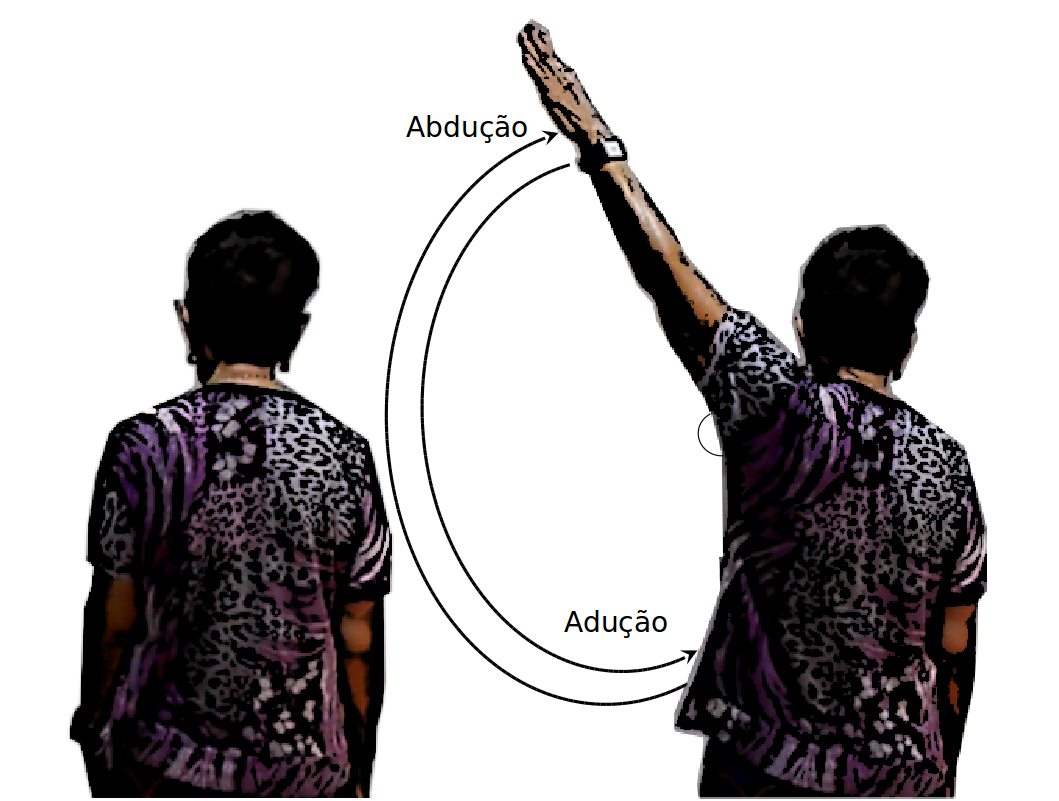
\includegraphics[scale=0.25]{./img/movaddcutctionartist2.png}
 % matrixargseg.png: 296x162 pixel, 100dpi, 7.52x4.11 cm, bb=0 0 213 117
 %\caption{Estágio desenvolvimento de jogos ~\cite{fullerton2008game}}
\caption{Movimentos de Abdução e Adução}
%  \caption{Estágio desenvolvimento de jogos}
 \label{fig:movabducaomet}
\end{figure}

Durante a análise foram comparados os Ângulos Relativos do Tronco e do Levantamento de Braços dos Indivíduos. As grandezas cinemáticas coletadas nesses estudo foram:
\begin{enumerate}
	\item Do movimento de abdução, a máxima amplitude atingida pelos membros superiores;
	\item velocidade angular de abdução membros esquerdo e direito;
	\item velocidade angular de adução membros esquerdo e direito.
\end{enumerate}

Os dados capturados desta fase resultaram na extração de características do movimento incluindo: a amplitude do movimento dos braços do lado esquerdo e direito, a velocidade angular dos movimentos de adução e abdução. A descrição dos vetores de características estão descritos na Tabela~\ref{table:features}.


\begin{table}[h]
\centering
\caption{Detalhamento do vetor de características extraído da coleta de dados.}
\label{table:features}
\begin{tabular}{|l|l|}
\hline
{\bf Característica}  & {\bf Descrição}                                       \\ \hline
MaxAmpEsquerdo     & Amplitude máxima do braço esquerdo. \\ \hline
MaxAmpDireito    & Amplitude máxima do braço direito. \\ \hline
AngVelAbdEsquerdo  & Velocidade angular do movimento de abdução do braço esquerdo. \\ \hline
AngVelAbdDireito & Velocidade angular do movimento de abdução do braço direito. \\ \hline
AngVelAdEsquerdo  & Velocidade angular do movimento de adução do braço esquerdo. \\ \hline
AngVelAdDireito & Velocidade angular do movimento de adução do braço direito. \\ \hline
\end{tabular}
\end{table}

\begin{figure}[!htb]
	\centering
	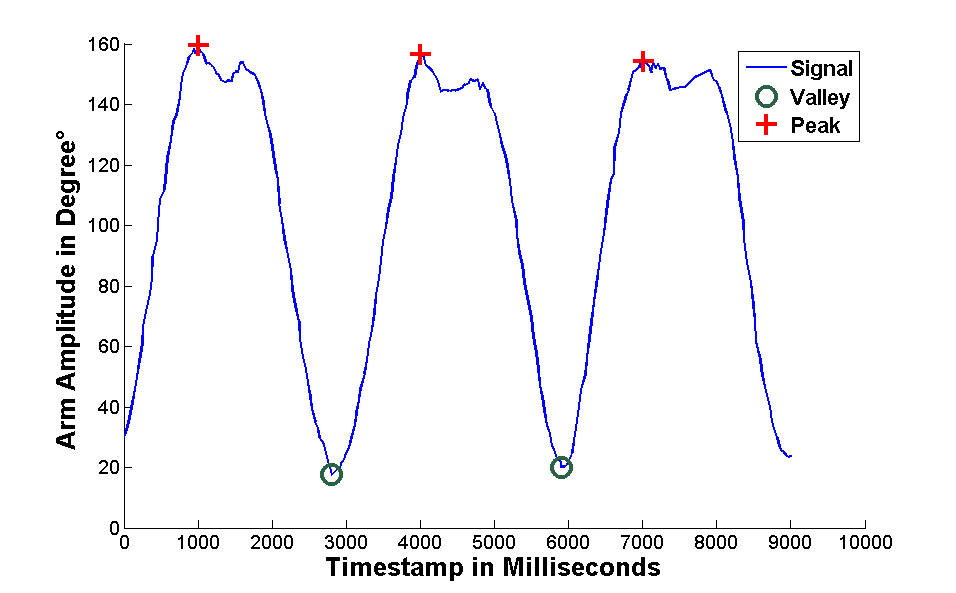
\includegraphics[width=1\textwidth]{img/signalamplitudepeakvaley-2.png}
	\caption{Exemplo do gráfico dos ângulos de adução e abdução dos braços em função do tempo}
	\label{fig:signalamplitudepeakvaley}
\end{figure}

A partir da extração das características do movimento, a próxima etapa da pesquisa é classificar os dados de movimento e identificar a ocorrência do sintoma de bradicinesia. Por meio das teorias estatísticas de aprendizagem de máquina, foi realizado uma análise dos dados para aquisição de conhecimento utilizando técnicas de aprendizagem supervisionada. 

%Logo, os dados biomecânicos~\cite{hamill1999bases} coletados foram utilizados com a \ac{dp} ante os indivíduos sem o diagnóstico estabelecido. Pelo quantitativo da pesquisa ter sido de 30 indivíduos, a abordagem de aprendizagem de máquina usando \ac{svm} ~\cite{vapnik95} foi utilizada juntamente com a técnica de validação-cruzada \textit{leave-one-out}, essa técnica será explicada com mais detalhes na Seção \ref{validacao_cruzada_svm}.


\subsubsection{Relação Risco e Benefício da Pesquisa}
Os riscos inerentes podem decorrer da exposição de dados dos sujeitos da pesquisa, o que pode acarretar danos morais e/ou psicológicos. Logo, teve-se um cuidado de preservar a integridade física e psicológica dos sujeitos da pesquisa, garantindo assim, a privacidade e confidencialidade das informações.

Caso houvesse algum constrangimento por parte do sujeito da pesquisa, ao não conseguir realizá-la ou responder alguma pergunta devido ao comprometimento da doença, os pesquisadores prestaram total assistência, orientando-o adequadamente para prosseguir ou encerrar o procedimento.

%Os presentes riscos fazem jus aos benefícios que a pesquisa venha a trazer com a possibilidade de monitoramento dos sinais da \ac{dp}. A identificação dos sinais motores e classificação desses dados através do computador podem permitir avanços para um melhor acompanhamento da evolução da doença além de possibilitar que os pacientes venham a ser monitorados de forma não invasiva através de um jogo eletrônico. Os pacientes deverão ter o seu estágio da \ac{dp} previamente diagnosticada por um médico para ser possível comparar os dados do monitoramento com a classificação obtida.




\subsection{Aplicação do Método}
O propósito da classificação é explorar a possibilidade de obter dados de saúde de forma contínua e não invasiva a partir de um sensor de captura de movimento usado em jogos eletrônicos (Ms-Kinnect). Durante a coleta dos dados foi indagado junto aos voluntários sua condição física e possíveis riscos e desconfortos que o voluntário pudesse ter ao realizar o procedimento. 

Durante a pesquisa, partiu-se do princípio, que através da análise do movimento de abdução e adução do braço, seria possível avaliar a biomecânica da amplitude do movimento dos braços e velocidade angular dos mesmos. Então, por intermédio desses dados biomecânicos, seria possível identificar a ocorrência do sintoma de bradicinesia em indivíduos portadores do \ac{dp}.



\subsection{Resultados}
Conforme a abordagem~\ac{jogue-me} apresentada no Capítulo~\ref{chapter:abordagem_gahme}, os dados adquiridos foram processados, extraídas as características do movimento angular, filtrados e postos em uma Máquina de Vetor de Suporte, para realizar a classificação entra as duas classes de dados. Para a classificação dos dados foi utilizado um \textit{kernel} Linear (Seção~\ref{sec:svm_linear}) por ter obtido os melhores resultados dentre os \textit{kernels} presentes no Matlab~\cite{matlab2011}: Polinomial, Radial e de MLP. O resultado do \textit{kernel} linear foi o mais expressivo entre os demais devido a separação linear ter dividido bem as duas classes. 

\subsubsection{Vetor Médio}
Nessa etapa da pesquisa foi calculado o Vetor Médio (Seção~\ref{section:filtro_dados}), para entender melhor a diferença de movimento entre os sujeitos diagnosticados com a \ac{dp} e sujeitos sem o diagnóstico. Como pode ser visto na Figura~\ref{fig:vetor_medio_abducao}, a amplitude de movimento de um indivíduo diagnosticado com ~\ac{dp} é bem menor do que a de um indivíduo sem o diagnóstico. Entretanto, por ter sido escalonado em 20 \textit{frames}, esse vetor médio perdeu a informação da velocidade do movimento.

\begin{figure}[!htbp]
 \centering
 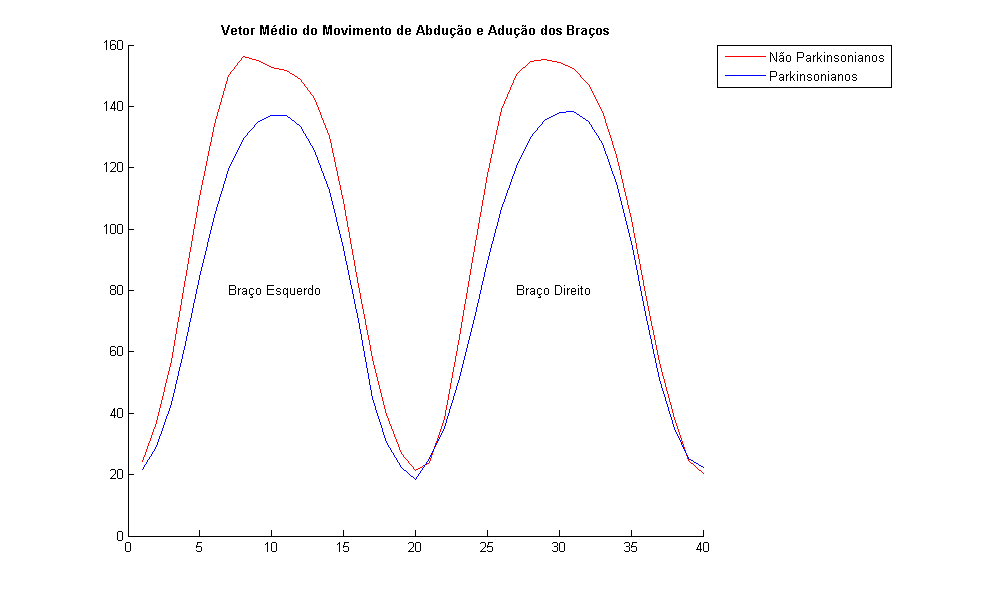
\includegraphics[scale=0.650]{./img/vetormedioaducao.png}
 \caption{Vetor Médio do Movimento de Abdução e Adução}
 \label{fig:vetor_medio_abducao}
\end{figure}

% 
% 
% \subsubsection{Validação Cruzada}\label{validacao_cruzada_svm}
% Para verificar a precisão da classificação de indivíduos saudáveis perante os parkinsonianos foi aplicada a técnica de Validação Cruzada (cross-validation) ~\cite{datamining2005}. A validação cruzada é uma técnica empregada para avaliar a capacidade de generalização de um modelo de predição em um conjunto de dados. Em um primeiro momento, realiza-se a partição do conjunto de dados em subconjuntos mutualmente exclusivos e ,posteriormente, usa-se este subconjunto para verificar a acurácia do modelo ~\cite{datamining2005}. 
% %O conceito central das técnicas de validação cruzada é o particionamento do conjunto de dados em subconjuntos mutualmente exclusivos, e posteriormente, usar alguns destes subconjuntos como dados de treinamento para encontrar valores que permitam a predição. O restante dos subconjuntos serão usados como dados de teste utilizados para avaliar o modelo preditivo.
% 
% A escolha do grupo de treinamento deve contemplar todas as classes no conjunto de dados, este procedimento é chamado de estratificação ou \textbf{Validação Cruzada Estratificada}~\cite{datamining2005}. Essa técnica é muito utilizada para mitigar a ocorrência de viés na pesquisa, pois o processo de treinamento é repetido por várias vezes com amostras diferentes incluindo diferentes casos em cada classe. Dada uma amostra única, um método de predição de taxa de erro na aprendizagem de máquina é usar a Validação-Cruzada dez vezes (\textit{10 K-Fold Cross-Validation})~\cite{datamining2005}, onde os dados são aleatórios e divididos em 10 grupos com a mesma proporção de classe. O processo de aprendizagem é executado por 10 vezes onde 1 grupo é selecionado como grupo de teste e os demais são selecionados como grupo de treinamento. A taxa de erro é calculada em cada processo de aprendizagem executado e no final é calculada a taxa de erro global. 
% 
% A escolha do número 10 para a quantidade de grupos não foi de forma aleatória, a literatura recomenda que sejam utilizados 10 grupos para obter a melhor estimativa de erro ~\cite{datamining2005}. Contudo, é reconhecido que esse número de 10 não é único ou insubstituível e em determinados casos, grupos de 5, 20 ou quaisquer outros números podem trazer melhores resultados.
% 
% Outro dado relevante para a escolha da técnica da estimativa de erro, é que uma única aplicação de Validação Cruzada \textit{10 K-Fold} pode não ser o suficiente para uma taxa de erro confiável. Pois, diferentes experimentos de Validação Cruzada podem produzir resultados distintos devido a natureza aleatória da escolha dos grupos. A estratificação reduz essa variação, contudo não a elimina completamente. Na busca por uma estimativa de erro mais exata, um procedimento que tem se transformado padrão nas técnicas de aprendizagem de máquina é repetir o processo de Validação Cruzada \textit{10 K-Fold} por 10 vezes. Ou seja, consiste em invocar o algoritmo de aprendizagem 100 vezes em um conjunto de dados, dessa forma aumenta-se a amostra de forma considerável e por consequência reduz-se a variação da taxa de erro na execução dos experimentos.
% 
% Desta maneira, o método escolhido de validação cruzada foi repetir e calcular por 10 vezes a \textit{10 K-Fold}. Os subjconjuntos são estratificados antes de cada um dos 10 processos de aprendizagem e a taxa de erro estimada em cada etapa processo de aprendizagem está exposta na Figura \ref{fig:erroestimadopca}. A taxa de classificação global é a média da taxa de acerto calculada em todo o processo.


\subsubsection{Matriz de Confusão e Suas Métricas}
Para avaliar o resultado da classificação, será apresentada a \textbf{matriz de confusão}~\cite{datamining2005}, que permite comparar os valores reais da classe com os valores obtidos no modelo de predição. 

A matriz de confusão para duas classes consiste numa matriz $2$\ x $2$\, contendo os \textit{Verdadeiros Positivos} (\textbf{TP}) e \textit{Verdadeiro Negativo} (\textbf{TN}), que são as classificações corretas. Os \textit{Falsos Negativos} (\textbf{FN}) contém a predição incorreta de um valor que deveria ser positivo e os \textit{Falsos Positivos} (\textbf{FP}) contém os valores positivos quando deveriam ser negativos como pode ser visto na Tabela~\ref{table:descricaomatrizconfusao}.

% Please remember to add \use{multirow} to your document preamble in order to suppor multirow cells
\begin{table}[!htbp]
\caption{Descrição da Matriz de Confusão}
\label{table:descricaomatrizconfusao}
\begin{tabular}{ll|c|c|}
\cline{3-4}
                                                                                                               & \multicolumn{1}{c}{}                         & \multicolumn{2}{|c|}{\textit{\textbf{Classe Preditiva}}} \\ \cline{3-4} 
                                                                                                               &                                              & \textbf{Parkinson}          & \textbf{Não Parkinson}     \\ \hline
\multicolumn{1}{|c}{\multirow{\textit{\textbf{\begin{tabular}[c]{@{}c@{}}Classe\\ Atual\end{tabular}}}}} & \multicolumn{1}{|l|}{\textbf{Parkinson}}     & Verdadeiros Positivos (VP)  & Falsos Negativos (FN)      \\ \cline{2-4} 
\multicolumn{1}{|l}{\textit{\textbf{}}}                                                                        & \multicolumn{1}{|l|}{\textbf{Não Parkinson}} & Falsos Positivo (FP) & Verdadeiros Negativos (VN) \\ \hline
\end{tabular}
\end{table}

% 
% A matriz de confusão é uma ferramenta importante para avaliar os resultados de predição, pois facilita o entendimento do que está sendo avaliado e como se comporta o classificador em relação aos erros de classificação obtidos. Esta matriz serve como base para métricas que podem ser aplicadas a classificação e,  consequentemente, exibem a precisão do modelo. A matriz desta pesquisa (Tabela ~\ref{table:resultadomatrizconfusaopca}) foi gerada a partir da repetição de dez vezes da técnica de Validação Cruzada \textit{10-K-Fold}, conforme a Seção \ref{sec:validacao_cruzada_database}.
% 
% \begin{table}[!htbp]
% \caption{Resultado da Matriz de Confusão}
% \label{table:resultadomatrizconfusaopca}
% \centering
% \begin{tabular}{l|c|c|}
% \cline{2-3}
% \multicolumn{1}{c}{}                         & \multicolumn{2}{|c|}{\textit{\textbf{Classe Preditiva}}} \\ \cline{2-3} 
%                                              & \textbf{Parkinson}      & \textbf{Não-Parkinson}         \\ \hline
% \multicolumn{1}{|l|}{\textbf{Parkinson}} & 429       & 71           \\ \hline
% \multicolumn{1}{|l|}{\textbf{Não Parkinson}}     & 114           & 386     \\ \hline
% \end{tabular}
% \end{table}
% 


\subsection{Aprendizagem de Máquina (SVM)}

Para uma base de dados pequena contendo 30 indivíduos, o método de Validação Cruzada escolhido deve tentar maximizar o conjunto de treinamento para atingir um melhor resultado de teste. Por esse motivo, foi escolhido o método de validação cruzada \textit{leave-one-out}. 

O método \textit{leave-one-out} é um método de validação cruzada \textit{k-fold} com o mesmo número de \textit{n} indivíduos. Logo, apenas um indivíduo será considerado teste e os demais serão de treinamento. Desta maneira não existe estratificação nos dados, tornando o processo determinístico e repetível com a mesma base de dados, pois não existe o problema de viés na seleção dos dados. A taxa de erro obtida da classificação é a taxa de erro do modelo para aquela base de dados. 

\subsubsection{Otimização dos Parâmetros da SVM - Método Grid-Search}

Para identificar os melhores parâmetros~\ac{svm}, foi aplicada a técnica~\cite{gridsearchsvm2010} usando validação cruzada \textit{Leave-One-Out} (LOOCV)~\cite{datamining2005}. Esta técnica avalia a precisão do modelo prevista , evita o problema superajuste na classificação binária e é um método prático para identificar os parâmetros SVM . Neste estudo, para reduzir a taxa de erro , nós aplicamos uma abordagem minimax para maximizar a margem sobre os coeficientes hiperplano ea classificação correta. Os valores dos parâmetros de pesquisa do \textit{grid-search} foi de: $C$ = [$2^5$, ... ,$2^2$] e $\gamma$ = [$2^{15}$, ... ,$2^3$ ] usando assim uma exponencial de base 2. Por meio desta técnica foi possível identificar uma região em que o classificador possuía a melhor acurácia e menor taxa de \textit{FpRate}. Após identificar essa região realizamos uma busca mais detalhada utilizando a técnica de \textit{grid-search} com os seguintes parâmetros: $C$ = [0.25, 0.5, ... ,2.5]; e $\gamma$ = [1, 2, ...,10] como 
pode ser visto na Figura~\ref{fig:gridaccuracy}.

%To identify the best SVM parameters, we applied the grid search technique~\citep{gridsearchsvm2010} using Leave-One-Out Cross-Validation (LOOCV)~\citep{datamining2005}. This technique assesses the accuracy of the predicted model, prevents the overfitting problem in the binary classification and is a practical method to identify the SVM parameters. In this study, to reduce the error rate, we applied a minimax approach to maximize the margin over the hyperplane coefficients and the correct classification. The parameters values of grid search for $C$ = [$2^5$, ... ,$2^2$] and $\gamma$ = [$2^{15}$, ... ,$2^3$ ], the step length was $2^2$, and with the identification and selection of a “better” region on the grid. So, we did a finer 


\begin{figure}[!h]
 \centering
 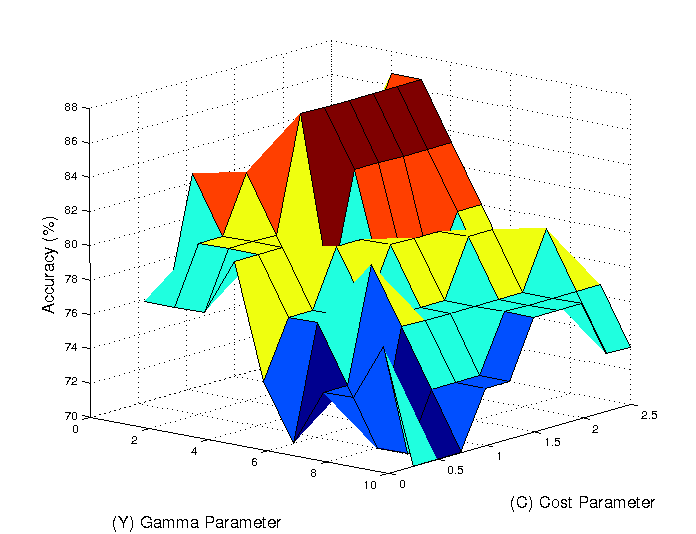
\includegraphics[scale=0.7]{./img/gridsearch.png}
 % matrixargseg.png: 296x162 pixel, 100dpi, 7.52x4.11 cm, bb=0 0 213 117
 %\caption{Estágio desenvolvimento de jogos ~\cite{fullerton2008game}}
\caption{\textit{Grid-Search} - Acurácia da Classificação}
%  \caption{Estágio desenvolvimento de jogos}
 \label{fig:gridaccuracy}
\end{figure}



% \begin{figure*}[htbp!]
% \subfigure[\textit{Grid-Search} - Acurácia da Classificação.]{
% 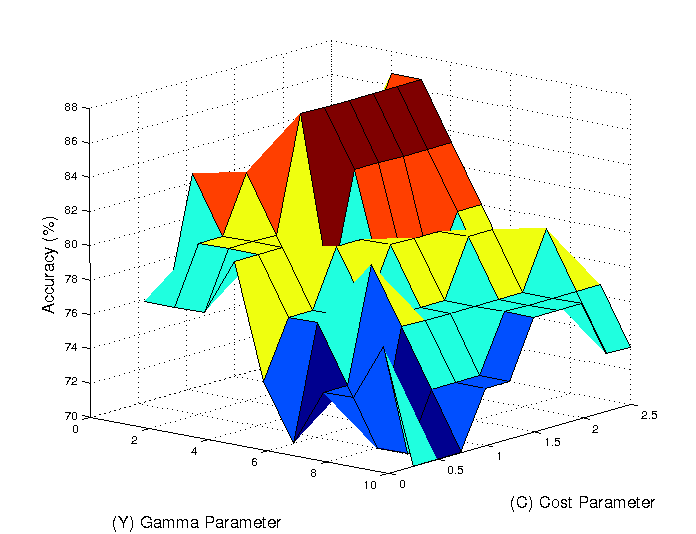
\includegraphics[scale=0.4]{./img/gridsearch.png}
% \label{fig:gridaccuracy}
% }
% \subfigure[Grid Search - FPRate.]{
% 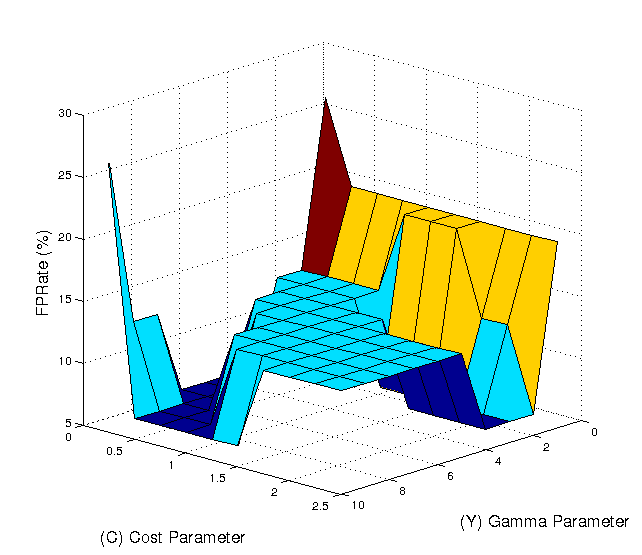
\includegraphics[scale=0.4]{./img/gridsearchfprate.png}
% \label{fig:gridfprate}
% }
% \label{fig:gridsearch}
% \caption{GridSearch for SVM Parameter Optimization.}
% \end{figure*}
% 
Como pode ser analisado na Figura~\ref{fig:gridaccuracy}, nós conseguimos uma classificação nos dados em que a pior seleção obteve uma acurácia de 70,00\% e melhor de 86,67\%. Conseguimos também um baixo valor de \textit{FpRate} com 6,67\% no melhor dos casos (Figura~\ref{fig:gridfprate}). Usando a técnica de \textit{grid-search} nós encontramos como melhor valor para os parâmetros: $C = 2$ and $\gamma = 3$. Como podemos analisar nos nossos resultados, por meio da técnica \textit{grid-search} foi possível identificar parâmetros para o classificador~\ac{svm} com uma boa generalização e que foi capaz de identificar a maior \textit{acurácia} e e menor nível de \textit{FpRate}.


\begin{figure}[!h]
 \centering
 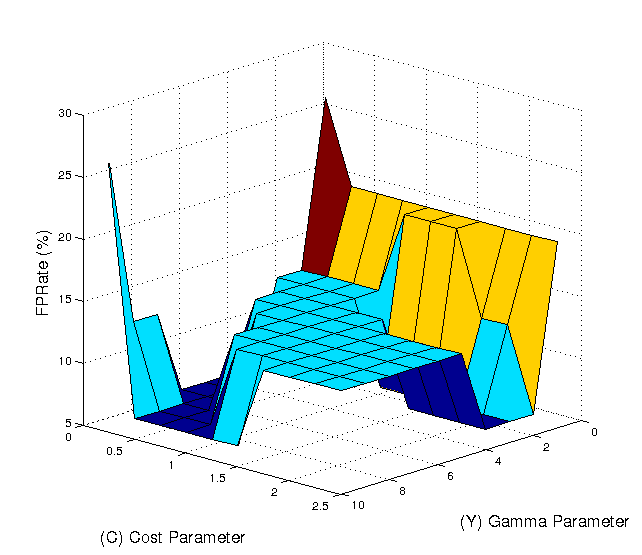
\includegraphics[scale=0.7]{./img/gridsearchfprate.png}
 % matrixargseg.png: 296x162 pixel, 100dpi, 7.52x4.11 cm, bb=0 0 213 117
 %\caption{Estágio desenvolvimento de jogos ~\cite{fullerton2008game}}
\caption{\textit{Grid-Search} - \textit{FpRate}}
%  \caption{Estágio desenvolvimento de jogos}
 \label{fig:gridfprate}
\end{figure}


%As illustrated in Fig.~\ref{fig:gridaccuracy}, we achieved a good classification performance where the worst accuracy was 70.00$\%$ and the best was 86.67$\%$. We obtained very low values for False Positives (FP), with 6.67$\%$ of \textit{FPRate} on the best fit (Fig.~\ref{fig:gridfprate}). This way, $C = 2$ and $\gamma = 3$ were the best kernel parameters, achieving accurate classification and minimizing the \textit{FPRate}. 

%The best classification performance of this study is presented in the confusion matrix for two classes that consist of a matrix $2$\ x $2$\, with (TP, FP, TN and FN) described in Table~\ref{table:resultadomatrizconfusaosvm}. True Positive (TP) indicates correctly classified with abnormal movement.  True Negative (TN) indicates correctly classified with normal movement. False Positives (FP) indicate the normal movement classified as abnormal ones and the False Negatives (FN) indicate the real abnormal movement not correctly detected. 

%Table~\ref{table:metricas} shows the classification performance, where the \textit{TpRate} is TP divided by the total number of positives, which is TP + FN; the \textit{FpRate} is FP divided by the total number of negatives, which is FP + TN. The \textit{Accuracy} is the number of correct classifications divided by the total number of classifications~\citep{datamining2005}.

%\subsection{Técnicas de Otimização da SVM}



%
%\begin{figure}
 %\centering
 %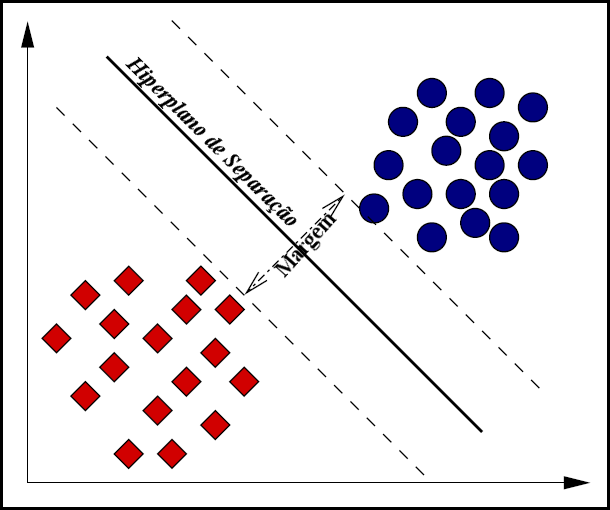
\includegraphics[scale=0.4]{./img/svmhyperplane.png}
 %% matrixargseg.png: 296x162 pixel, 100dpi, 7.52x4.11 cm, bb=0 0 213 117
 %%\caption{Estágio desenvolvimento de jogos ~\cite{fullerton2008game}}
%\caption{Hiperplano de Separação Linear Para Duas Classes}
%%  \caption{Estágio desenvolvimento de jogos}ETAPA 3 - Avaliação Da Aceitação Da Abordagem Junto aos Pacientes de~\ac{dp} Utilizando \textit{Goal Question Metric}
 %\label{fig:hiperplano}
%\end{figure}
%
%
%
%
%A aprendizagem supervisionada consiste em que dado um conjunto de dados para treinamento 
%
%O modelo mais simples de ~\ac{svm},foi o primeiro a ser desenvolvido, foi chamado de Classificador de Margem Máxima, o qual trabalha apenas com dados linearmente separáveis, ficando restrito a essas aplicações. Contudo, apesar dessa restrição o Classificador de Margem Máxima possui propriedades importante que foram fundamentais para a elaboração de SVMs mais eficazes ~\cite{svm-cg-2002}. 
%
%\begin{figure}
 %\centering
 %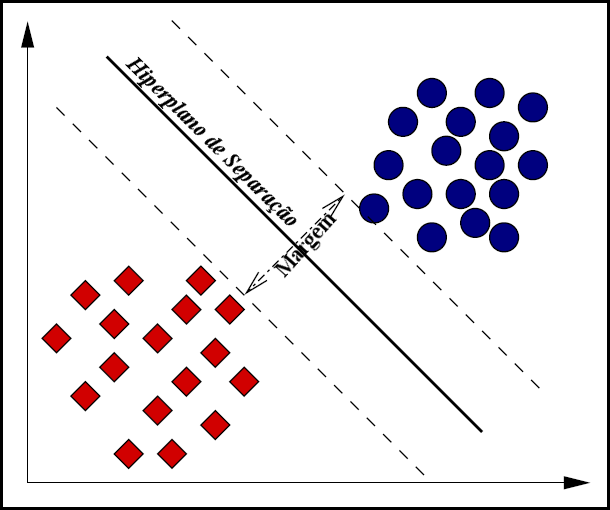
\includegraphics[scale=0.4]{./img/svmhyperplane.png}
 %% matrixargseg.png: 296x162 pixel, 100dpi, 7.52x4.11 cm, bb=0 0 213 117
 %%\caption{Estágio desenvolvimento de jogos ~\cite{fullerton2008game}}
%\caption{Hiperplano de Separação Linear Para Duas Classes}
%%  \caption{Estágio desenvolvimento de jogos}
 %\label{fig:hiperplano}
%\end{figure}
%
%Pode ser visto na Figura ~\ref{fig:hiperplano_linear_separavel} uma projeção de dados bidimensionais temos a representação de um conjunto de dados de treinamento  bidimensional e sua separação linear a separação dos dados pode ser realizada linearmente 
%
%\begin{figure}
 %\centering
 %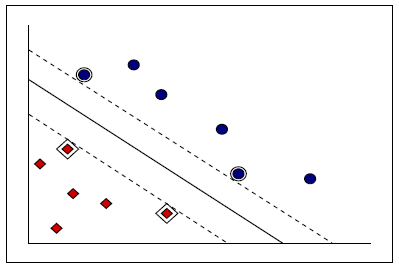
\includegraphics[scale=0.4]{./img/hiperplano-linear.png}
 %% matrixargseg.png: 296x162 pixel, 100dpi, 7.52x4.11 cm, bb=0 0 213 117
 %%\caption{Estágio desenvolvimento de jogos ~\cite{fullerton2008game}}
 %\caption{Espaço de Características Linearmente Separável ~\cite{svm-cg-2002}}
%%  \caption{Estágio desenvolvimento de jogos}
 %\label{fig:hiperplano_linear_separavel}
%\end{figure}
%
%\begin{figure}
 %\centering
 %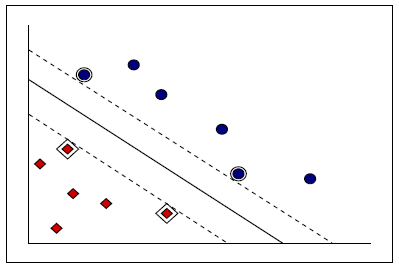
\includegraphics[scale=0.4]{./img/hiperplano-linear.png}
 %% matrixargseg.png: 296x162 pixel, 100dpi, 7.52x4.11 cm, bb=0 0 213 117
 %%\caption{Estágio desenvolvimento de jogos ~\cite{fullerton2008game}}
 %\caption{Espaço de Características Linearmente Inseparável ~\cite{svm-cg-2002}}
%%  \caption{Estágio desenvolvimento de jogos}
 %\label{fig:linear-inseparavel}
%\end{figure}
%
%
%
%% Vapnik idealizou o princípio indutivo de Minimização do Risco Estrutural. Este princípio busca minimizar o erro do conjunto de treinamento (risco empírico), juntamente com o erro do conjunto de teste \cite{svm-cg-2002}.
%
%Formalmente, classificadores que separam os dados por meio de um hiperplano de Equação(~\ref{eq:hiperplano}) são denominados discriminante linear~\cite{valt2010}.
%\linebreak
%\begin{equation}
%f(x)=w^Tx+b=0
%\label{eq:hiperplano}
%\end{equation}.



\subsubsection{Resultados Obtidos}
A Matriz de Confusão obtida indica que existem três indivíduos classificados como ``Não-Parkinson'' e que possuem a doença, no entanto analisando as características do movimento desses indivíduos ``Parkinsonianos'' percebemos que eles possuíam uma amplitude de movimento e uma velocidade angular bastante próximas dos indivíduos do Grupo Controle. Logo, estes não apresentam o sintoma de bradicinesia, o que pode indicar que o indivíduo esteja no início da doença, ou bem medicado, ou inclusive não apresentar este sinal motor o que está adequada a sintomatologia do~\ac{dp}. 
Um resultado, que não era esperado nesta pesquisa é a ocorrência de um indivíduo que não possui~\ac{dp} mas mesmo assim foi classificados com o sintoma. Analisando seus dados foi percebido que ele possuía sinais muito próximos do grupo dos indivíduos com~\ac{dp}, logo ele possivelmente apresenta algum déficit motor o que condiz com o resultado da classificação.

\begin{table}[!htbp]
\caption{Resultado da Matriz de Confusão SVM}
\label{table:resultadomatrizconfusaosvm}
\centering
\begin{tabular}{l|c|c|}
\cline{2-3}
\multicolumn{1}{c}{}                         & \multicolumn{2}{|c|}{\textit{\textbf{Classe Preditiva}}} \\ \cline{2-3} 
                                             & \textbf{Parkinson}      & \textbf{Não-Parkinson}         \\ \hline
\multicolumn{1}{|l|}{\textbf{Parkinson}} & 12       & 3           \\ \hline
\multicolumn{1}{|l|}{\textbf{Não Parkinson}}     & 1           & 14     \\ \hline
\end{tabular}

\end{table}


 Para demonstrar a avaliação do modelo de forma quantitativa usou-se um conjunto de métricas derivadas da matriz de confusão ~\cite{datamining2005}.
 \begin{description}
 	\item [\textit{TpRate}] taxa de acerto obtido: $ TpRate = TP/P $\ ;
 	\item [\textit{FpRate}]: taxa de falso alarme obtido: $ FpRate = FP/N $\ ;
 	\item [\textit{Precision}]: taxa de acerto de uma instância em determinada classe: $ Precision =  TP/(TP +FP) $\ ;
 	\item [\textit{Accuracy}]: taxa de acerto de todo o classificador: $ Accuracy = (TP+TN)/(P+N) $\ ;
 	\item [\textit{F-Measure}]: análise de classificador binário que mede a acurácia do teste. Considerando a média harmônica da taxa de \textit{precision} e do \textit{tp rate}: $ F-Measure = 2 * (Precision * TpRate)/(Precision + TpRate) $\ .
 \end{description}



\begin{table}[!htbp]
\label{table:metricasmatrizconfusao}
\caption{Métricas da Matriz de Confusão}
\centering
\begin{tabular}{|l|r|}
\hline
\multicolumn{2}{|l|}{\textbf{Métricas}} \\ \hline
\textbf{TpRate}                    & 80,00$\%$\                 \\ \hline
\textbf{FpRate}                    & 6,67$\%$\                \\ \hline
\textbf{Precision}                 & 92,31$\%$\                \\ \hline
\textbf{Accuracy}                  & 86,67$\%$\                \\ \hline
\textbf{F-Measure}                 & 85,71$\%$\                \\ \hline
\end{tabular}
\end{table}






\subsubsection{Limitações do Método}
O método utilizado para diferenciar os movimentos executados de indivíduos diagnosticados com \ac{dp} ante os indivíduos sem o diagnóstico estabelecido, foi uma técnica estatística de aprendizagem denominada de~\ac{svm}. Nesse estudo não se pretende estabelecer um diagnóstico da \ac{dp}, ou até mesmo provar que os movimentos utilizados pelos participantes da pesquisa servem para um diagnóstico. Contudo, este trabalho demonstra que existem diferenças entre essas duas classes, e estas podem ser capturadas por um sensor de movimento usado em jogos eletrônicos, e que essas diferenças podem ser classificadas utilizando uma abordagem de aprendizagem de máquina. 

\section{ETAPA 3 - Avaliação Da Aceitação Da Abordagem Junto aos Pacientes de~\ac{dp} Utilizando \textit{Goal Question Metric}}\label{gqm_usuarios}
%Para identificar a possibilidade de integrar o monitoramento da saúde do jogador através de jogos eletrônicos à sua rotina diária, foi utilizada a abordagem \textit{Goal, Question, Metric} (GQM). GQM ~\cite{basili94} é uma abordagem hierárquica que inicia com objetivo principal e o divide em atividades que podem ser mensuradas durante a execução do projeto. É uma abordagem para integrar objetivos a e perspectivas de qualidade de interesse, baseado nas necessidades do projeto~\cite{van1999goal}. Foi preparado o questionário GQM mostrado no Apêndice~\ref{apend:gqm} para avaliar a possibilidade de monitorar dados motores de forma não invasiva e integrada a rotina diária das pessoas.

Com o objetivo de averiguar a possibilidade de integrar o monitoramento da saúde do jogador através de jogos eletrônicos à sua rotina diária, foi utilizada a abordagem \textit{Goal, Question, Metric} (GQM)~\cite{van1999goal}. Essa abordagem é um paradigma de pesquisa utilizado na Engenharia de Software para medição de processos de software e melhoria contínua dos produtos ~\cite{saraiva2006,elicquest05}. A qualidade do produto de software~\cite{saraiva2006} pode ser compreendida como a adequação a um conjunto de características atingidas em maior ou menor grau para que o produto final venha atender as necessidades do usuário final, identificadas na fase de elicitação de requisitos ~\cite{elicquest05}.

O~\ac{gqm} é um paradigma de avaliação orientado por metas e tem como componentes elementares: objetivos, questionamentos e a métricas ~\cite{saraiva2006}. Nesse paradigma de pesquisa é definido um objetivo principal, onde são refinados em perguntas que venham extrair as métricas da pesquisa que fornecem informações. De posse das respostas baseada em métricas, estas são comparadas com o objetivo da pesquisa no intuito de identificar se ele foi alcançado. Logo, o paradigma~\ac{gqm} busca definir métricas partindo de uma perspectiva de ``de cima para baixo''; analisa, interpreta e mensura dados de maneira ``de baixo para cima'' como pode ser graficamente visualizado na Figura~\ref{fig:gqm} ~\cite{van1999goal}. 

\begin{figure}[!htbp]
 \centering
 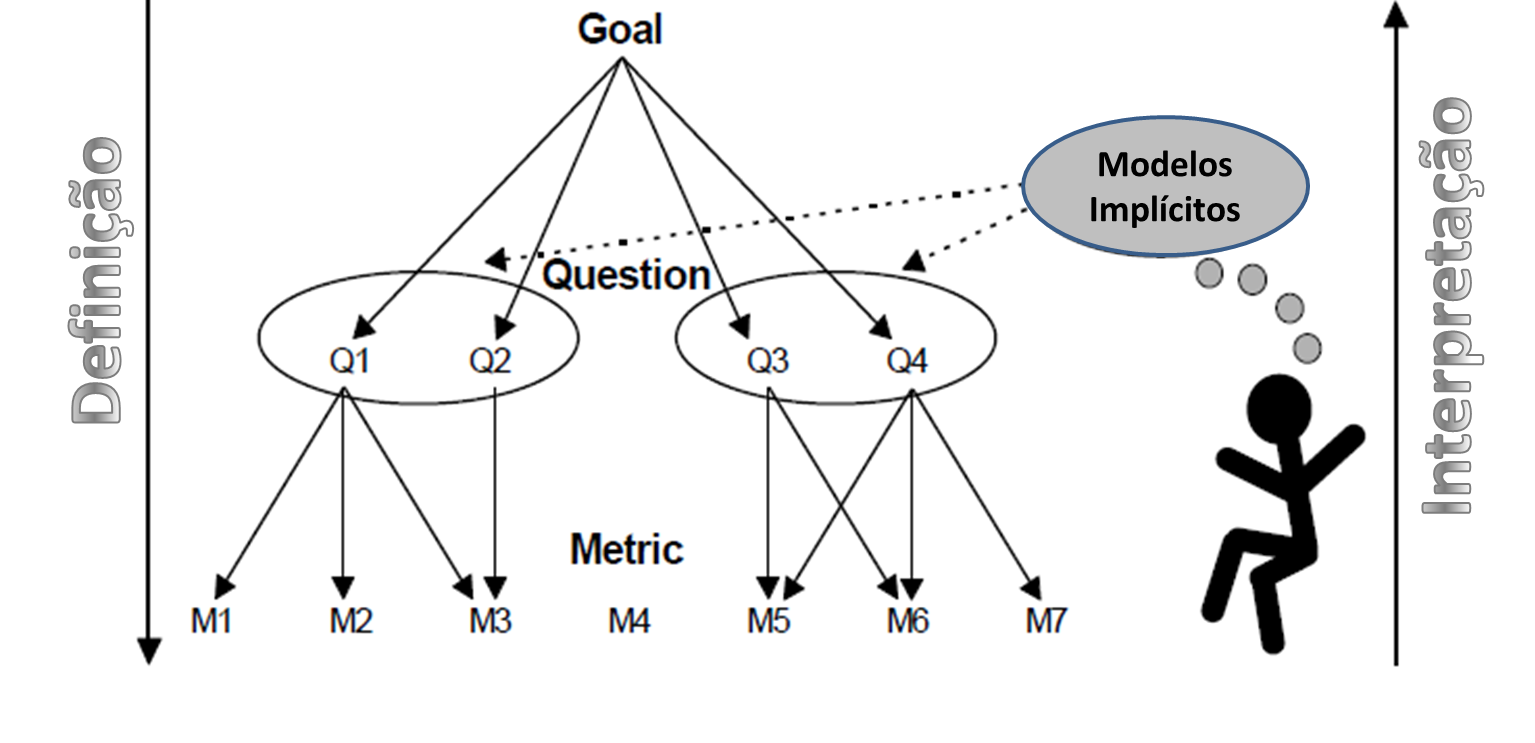
\includegraphics[scale=0.50]{./img/gqm.png}
 \caption[O Paradigma GQM \copyright]{O Paradigma GQM \copyright~\cite{van1999goal}}
 \label{fig:gqm}
\end{figure}

Segundo Saraiva ~\cite{saraiva2006}, numa análise da aplicação do método de ~\ac{gqm} para o contexto de avaliação de usabilidade de software, os componentes elementares do paradigma ~\ac{gqm} são:

\begin{itemize}
	\item \textbf{Objetivo}: Sua definição envolve o propósito da avaliação, o que deve ser avaliado, a perspectiva e o ambiente proposto.
	\item \textbf{Questão}: A questão anuncia a necessidade de se obter informações em linguagem natural, podendo formular uma ou mais questões para cada categoria. Logo, sua resposta deve estar condicionada ao objetivo proposto.
	\item \textbf{Métrica}: Sua função é especificar os dados que se deseja obter durante as avaliações em termos quantitativos, podendo ter mais de uma métrica para cada questão.	
\end{itemize}

Baseado nos componentes elementares do paradigma, foi elaborado um questionário~\ac{gqm} (Apêndice~\ref{apend:gqm}) com o objetivo principal de avaliar a possibilidade de monitorar dados motores, de forma não invasiva e integrada a rotina diária dos usuários. Para elaboração de métricas para atingir esse objetivo foram formuladas duas questões de pesquisa com o intuito de avaliar:
\begin{enumerate}
	\item se o usuário integraria a abordagem~\ac{jogue-me} à sua rotina diária;
	\item se a segurança com a integridade física está de acordo com a faixa etária do usuário.
\end{enumerate}

O questionário consistiu de um conjunto de 10 questões de resposta fechada (quantitativa) ~\cite{elicquest05}, e o entrevistado deve escolher uma resposta dentre as alternativas dadas. Esse método foi escolhido para contribuir por uma maior uniformidade nas respostas e consequentemente facilitar sua análise. Porém, este método impede a expressão das opiniões dos entrevistados~\cite{elicquest05}. 

%\begin{table}
%\begin{longtable}{|p{\textwidth}|}
%\caption{O Questionário GQM}\\
%\label{table:table_gqm}
%\hline
%\endfirsthead
%\multicolumn{1}{c}%
%{\tablename\ \thetable\ -- \textit{Continuação da página anterior}} \\
%\hline
%\endhead
%\hline \multicolumn{1}{r}{\textit{Continua na próxima página}} \\
%\endfoot
%\hline
%\endlastfoot
%\textbf{\textit{Objetivo principal}}: Avaliar a possibilidade de monitorar dados motores de forma não invasiva e integrada a rotina diária das pessoas. \\ \hline
%\textbf{\textit{Questão 1}}: O usuário poderia integrar a abordagem \textit{HGMS-E} à sua rotina diária ?\\ \hline
%\textit{Métrica 1.1}: Numa escala de 1 a 5 qual o grau de diversão do jogo? \\ \hline
%\textit{Métrica 1.2}: O jogo traz motivação ao usuário ? (Sim/Não) \\ \hline
%\textit{Métrica 1.3}: Se o usuário tivesse adquirido esse jogo, com que frequência o utilizaria durante a semana? (1 vez/3 vezes/Todos os dias/Nunca usaria) \\ \hline
%\textit{Métrica 1.4}: O usuário considera o jogo simples, sem muitas regras e de fácil entendimento ? Ele pode ser aplicado em diferentes idades? (Sim/ Não) \\ \hline
%\textit{Métrica 1.5}: O usuário tem o costume de jogar esses jogos casuais em casa? (Sim/ Não) \\ \hline
%\textit{Métrica 1.6}: O usuário agregaria um jogo desse estilo em sua rotina diária? (Sim/ Não) \\ \hline
%\textbf{\textit{Questão 2}}: A segurança com a integridade física está de acordo com a faixa etária do usuário ? \\ \hline
%\textit{Métrica 2.1}: Uma criança estaria segura jogando esse jogo, ao efetuar os movimentos dos braços? \\ \hline
%\textit{Métrica 2.2}: Um adulto estaria seguro ao jogar esse jogo, ao efetuar os movimentos dos braços? \\ \hline
%\textit{Métrica 2.3	}: Um idoso estaria seguro ao jogar esse jogo, ao efetuar os movimentos dos braços? \\ \hline
%\textit{Métrica 2.4}: Qual opinião do usuário sobre a faixa etária do jogo? (Livre/Crianças/Adultos/Idosos) \\ \hline
%\end{longtable}
%\end{center}
%\end{table}


\subsection{Aplicação do Método}
%A abordagem de ~\ac{GQM}, tem o intuito de auxiliar na elaboração de planos de avaliação de atributos de qualidade de produtos e processos de software ~\cite{basili94}. Sabemos, que essa abordagem é muito mais empregada na avaliação de processos, porém nessa pesquisa iremos invocar a técnica para a avaliação do produto do ponto de vista do usuário. Essa abordagem, permite identificar métricas apropriadas ao contexto e objetivos da avaliação de modo a facilitar a interpretação e análise dos dados orientados por metas.
%
%Essa etapa da pesquisa teve como objetivo avaliar se os possíveis usuários do sistema iriam aprovar o monitoramento motor usando jogos eletrônicos. Essa avaliação vai ao encontro do usuário final e principal beneficiado pela abordagem apresentada nessa proposta de Tese.

%Essa etapa da pesquisa foi realizada em colaboração com o trabalho de Santos Jr. ~\cite{antonio2013}, que desenvolveu também o mecanismo de captura dos dados Seção~\ref{sec:cliente_game}.  Tendo como objetivo avaliar se possíveis usuários do sistema iriam aprovar o monitoramento motor usando jogos eletrônicos. Essa avaliação vai ao encontro do usuário final e principal beneficiado pela abordagem apresentada nessa proposta de Tese.

Nessa etapa da pesquisa foram entrevistadas 24 pessoas do Laboratório Embedded da Universidade Federal de Campina Grande, do Instituto Federal de Alagoas, e em pacientes da Fundação Pestalozzi e da clínica de Fisioterapia do CESMAC (ambas em Maceió). Os usuários foram selecionados para jogar o \emph{Catch the Spheres} (Seção ~\ref{jogo_catch}), testaram e responderam o questionário para verificar a aceitabilidade da solução junto aos usuários. 

%Buscou-se também validar a viabilidade da Arquitetura de Software do \textit{\textit{HGMS-E}}, verificando a possibilidade de capturar dados motores. 
O procedimento para executar as sessões de teste foi:
\begin{enumerate}
	\item O usuário se posicionou a uma distância de 2 metros do sensor de movimento, de modo a adquirir toda a extensão superior do braço; 	
	\item O usuário iniciou o jogo \textit{Catch the Spheres}, conforme a interface da aplicação;
	\item O usuário utilizou o jogo \textit{Catch the Spheres} por volta de 00:01:30s;
	\item O usuário fechou a aplicação.
\end{enumerate}

\subsection{Resultados}
Os resultados do questionário são apresentados na Tabela ~\ref{table:resultados_gqm} contendo as respostas binárias ``Sim/Não'' e nas Figuras~\ref{fig:question1},\ref{fig:question3},\ref{fig:question10} nas perguntas de questões com múltipla escolha.

\textit{Questão 1 - O usuário poderia integrar a abordagem~\ac{jogue-me} à sua rotina diária ?}: os 24 usuários deram as seguintes respostas nas Métricas (1.1, 1.2, 1.3,1.4,1.5 e 1.6): 75\% dos usuário atribuíram ao menos nota 4 (de 1 a 5) ao grau de diversão do jogo; 91,67\% sentiram motivados com o jogo; 58\% dos usuários jogariam 3 vezes por semana, 25\% jogariam todos os dias e apenas 17\% jogariam uma vez por semana. 

Então, tem-se um percentual de 83\% de usuários que poderiam integrar o monitoramento motor a sua rotina; 91,67\% consideraram o jogo simples e de fácil entendimento, e isso permite o uso de um maior número de usuários. Uma métrica desfavorável foi que apenas 41,67\% dos usuários possuem o costume de usar jogos casuais em casa. Mas, devido a expectativa de melhora do estado de saúde, 75\% dos usuários responderam que agregariam o jogo a sua rotina diária.

\textit{Questão 2 - A segurança com a integridade física está de acordo com a faixa etária do usuário
?}: nesta questão percebe-se uma grande preocupação dos usuários quanto a risco de quedas. Inicialmente, a pesquisa seria destinada para o movimento de braços e pernas. Devido aos riscos, foi modificada para movimentação somente dos braços, reduzindo a preocupação dos usuários. Mesmo assim, as métricas obtidas demonstraram que o jogo é seguro para crianças e adultos. No caso dos idosos, 75\% dos usuários consideraram o jogo seguro para essa faixa etária, muito embora os mesmos usuários classificaram o jogo com a faixa etária ``livre'', com 88\% de ocorrência.

% Please remember to add \use{multirow} to your document preamble in order to suppor multirow cells
\begin{table}[h]
\caption{Métricas Avaliadas do \textit{GQM}}
\centering
\begin{tabular}{|p{10cm}|p{1.2cm}|p{1.2cm}|}
\hline
\textbf{Métrica} & \textbf{Sim} & \textbf{Não} \\ \hline
1.2: O jogo traz motivação ao usuário? & 91,67\% & 8,33\% \\ \hline
1.4: O usuário considera o jogo simples, sem muitas regras e de fácil entendimento? Ele pode ser aplicado em diferentes idades? & 91,67\% & 8,33\% \\ \hline
1.5: O usuário tem o costume de jogar esses jogos casuais em casa? & 41,67\% & 58,33\% \\ \hline
1.6: O usuário agregaria um jogo desse estilo em sua rotina diária? & 75\% & 25\% \\ \hline
2.1: Uma criança estaria segura jogando esse jogo, ao efetuar os movimentos dos braços? & 100\% & 0\% \\ \hline
2.2: Um adulto estaria seguro ao jogar esse jogo, ao efetuar os movimentos dos braços? & 100\% & 0\% \\ \hline
2.3: Um idoso estaria seguro ao jogar esse jogo, ao efetuar os movimentos dos braços? & 75\% & 25\% \\ \hline
\end{tabular}
\label{table:resultados_gqm}
\end{table}


\begin{figure}[!htb]
     \centering
     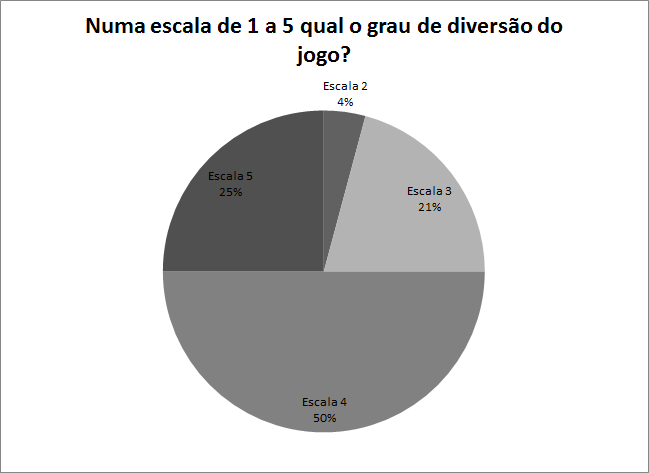
\includegraphics[scale=0.7]{./img/chart_1-.png}
     \caption{Resultado da Pergunta 1}
     \label{fig:question1}
\end{figure}


\begin{figure}[!htb]
     \centering
     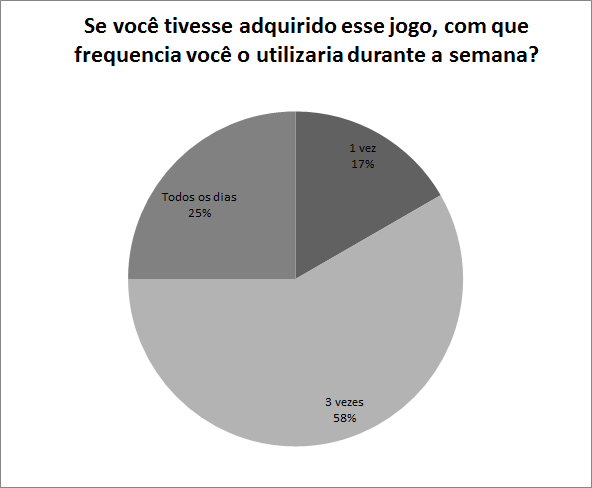
\includegraphics[scale=0.7]{./img/chart_3-.png}
     \caption{Resultado da Pergunta 3}
     \label{fig:question3}
\end{figure}


\begin{figure}[!htb]
     \centering
     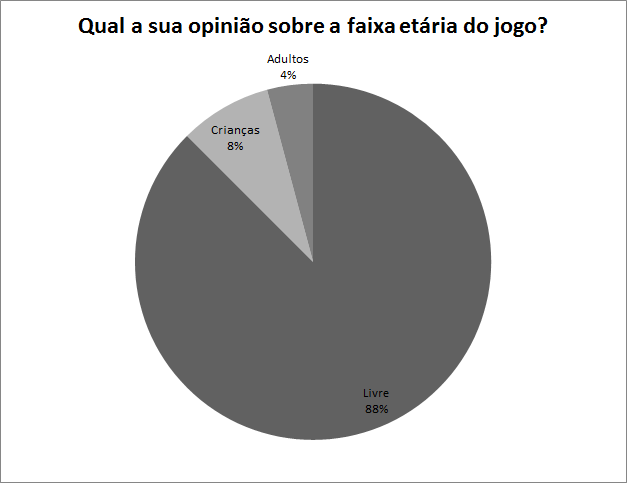
\includegraphics[scale=0.7]{./img/chart_10-.png}
     \caption{Resultado da Pergunta 10}
     \label{fig:question10}
\end{figure}
\FloatBarrier




%\begin{figure}
        %\centering
        %\begin{subfigure}[b]{0.3\textwidth}
                %\centering
                %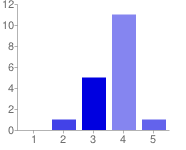
\includegraphics[width=\textwidth]{./img/chart_1.png}
                %\caption{Pergunta 1 (1: 0\%; 2: 6\%; 3: 28\%; 4: 61\%; 5: 6\%)}
                %\label{fig:question1}
        %\end{subfigure}%
        %~ %add desired spacing between images, e. g. ~, \quad, \qquad etc.
          %%(or a blank line to force the subfigure onto a new line)
        %\begin{subfigure}[b]{0.3\textwidth}
                %\centering
                %\includegrapResultado Obtidoshics[width=\textwidth]{./img/chart_2.png}
                %\caption{Pergunta 2 (Sim: 67\%; Não: 33\%)}
                %\label{fig:question2}
        %\end{subfigure}
        %~
        %\begin{subfigure}[b]{0.3\textwidth}
                %\centering
                %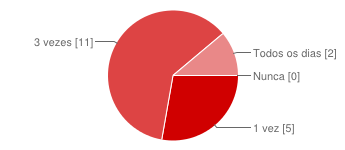
\includegraphics[width=\textwidth]{./img/chart_3.png}
                %\caption{Pergunta 3 (1 vez: 28\%; 3 vezes: 61\%; Todos os dias: 11\%; Nunca: 0\%)}
                %\label{fig:question3}
        %\end{subfigure}
%
        %\begin{subfigure}[b]{0.3\textwidth}
                %\centering
                %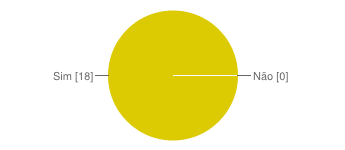
\includegraphics[width=\textwidth]{./img/chart_4.png}
                %\caption{Pergunta 4 (Sim: 100\%)}
                %\label{fig:question4}
        %\end{subfigure}
        %~
        %\begin{subfigure}[b]{0.3\textwidth}
                %\centering
                %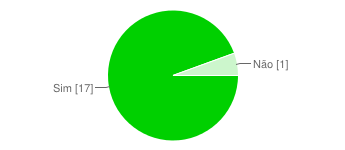
\includegraphics[width=\textwidth]{./img/chart_5.png}
                %\caption{Pergunta 5 (Sim: 94\%; Não: 6\%)}
                %\label{fig:question5}
        %\end{subfigure}
        %~
        %\begin{subfigure}[b]{0.3\textwidth}
                %\centering
                %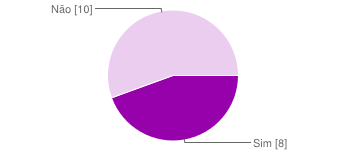
\includegraphics[width=\textwidth]{./img/chart_6.png}
                %\caption{Pergunta 6 (Sim: 44\%; Não: 56\%)}
                %\label{fig:question6}
        %\end{subfigure}
%
        %\begin{subfigure}[b]{0.3\textwidth}
                %\centering
                %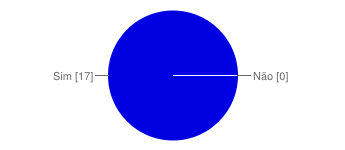
\includegraphics[width=\textwidth]{./img/chart_7.png}
                %\caption{Pergunta 7 (Sim: 100\%)}
                %\label{fig:question7}
        %\end{subfigure}
        %~
        %\begin{subfigure}[b]{0.3\textwidth}
                %\centering
                %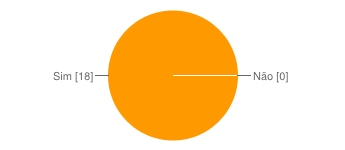
\includegraphics[width=\textwidth]{./img/chart_8.png}
                %\caption{Pergunta 8 (Sim: 100\%)}
                %\label{fig:question8}
        %\end{subfigure}
        %~
        %\begin{subfigure}[b]{0.3\textwidth}
                %\centering
                %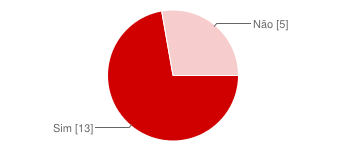
\includegraphics[width=\textwidth]{./img/chart_9.png}
                %\caption{Pergunta 9 (Sim: 72\%; Não: 28\%)}
                %\label{fig:question9}
        %\end{subfigure}
%
        %\begin{subfigure}[b]{0.3\textwidth}
                %\centering
                %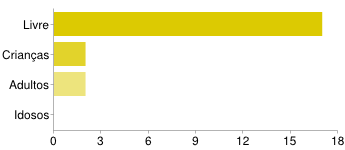
\includegraphics[width=\textwidth]{./img/chart_10.png}
                %\caption{Pergunta 10 (Livre: 80\%; Crianças: 10\%; Adultos: 10\%; Idosos: 0\%)}
                %\label{fig:question10}
        %\end{subfigure}
        %~
        %\begin{subfigure}[b]{0.3\textwidth}
                %\centering
                %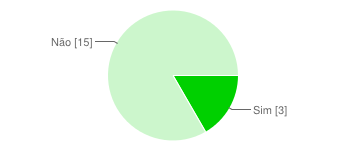
\includegraphics[width=\textwidth]{./img/chart_11.png}
                %\caption{Pergunta 11 (Sim: 17\%; Não: 83\%)}
                %\label{fig:question11}
        %\end{subfigure}
        %\caption{Gráficos das Respostas do questionário}\label{result}
%\end{figure}

\subsection{Conclusão} 
Nessa etapa, buscou-se demonstrar que podemos desenvolver um jogo com mecanismos de captura de dados motores embutidos e que permita monitorar e quantificar sinais do Parkinson de uma maneira não-invasiva. 

Apesar do questionário ter avaliado a opinião dos jogadores quanto ao jogo apresentado, pode-se generalizar que as opiniões são válidas para outros jogos usando a abordagem~\ac{jogue-me}. Deve-se levar em consideração, também, que as métricas obtidas nessa pesquisa foram extraídas de um jogo na fase de protótipo. Caso ele fosse aperfeiçoado é possível que sua aceitabilidade seria ainda maior. Por esse motivo, o resultado obtido com a pesquisa~\ac{gqm} foi positivo, e considera-se que é viável desenvolver um jogo com o objetivo de monitorar dados motores, de forma não invasiva, e integrada à rotina diária dos usuários.



